\documentclass[11pt]{report}
\usepackage{fancyhdr}
\usepackage{lastpage}
\usepackage{extramarks}
\usepackage{graphicx}
\usepackage{amsmath}
\usepackage[normalem]{ulem}
%% Please revise the following command, if your babel
%% package does not support en-US
\usepackage[english]{babel}
\usepackage{color}
\usepackage{hyperref}
\usepackage{pgffor}
\usepackage{filecontents}% Used so that the external files can be placed in this file
\usepackage{multicol}
\usepackage{color}
\usepackage{nicefrac}
\usepackage{lmodern}
\usepackage{gensymb}
\usepackage{titlesec}

%[nowarnings]
\usepackage{xcookybooky}
\usepackage[Conny]{fncychap}
% Bjornstrup

% Margins
%\topmargin=-0.5in
\evensidemargin=0in
\oddsidemargin=0in
%\textwidth=7.5in
%\textheight=9.0in
%\headsep=0.25in 

% command to provide stretchy vertical space in proportion
\newcommand\nbvspace[1][3]{\vspace*{\stretch{#1}}}
% allow some slack to avoid under/overfull boxes
\newcommand\nbstretchyspace{\spaceskip0.5em plus 0.25em minus 0.25em}
% To improve spacing on titlepages
\newcommand{\nbtitlestretch}{\spaceskip0.6em}

\newcommand{\newrecipe}{{\newpage}}

%\begin{titlepage}
%\title{Recipes}
%\author{The Hickson Family}
%\date{December 2019}
%\end{titlepage}

\titleclass{\part}{top} % make part like a chapter
\titleformat{\part}
[display]
{\centering\normalfont\Huge\bfseries}
{\titlerule[5pt]\vspace{3pt}\titlerule[2pt]\vspace{3pt}\MakeUppercase{\partname} \thepart}
{0pt}
{\titlerule[2pt]\vspace{1pc}\huge\MakeUppercase}
%

\begin{document}
%\maketitle

\begin{titlepage}
\begin{center}
\bfseries
\nbvspace[1]
\Huge
{\nbtitlestretch\huge
Hickson Family Recipes}

\nbvspace[1]
\normalsize

Family Recipes\\
Collected Together
\nbvspace[1]
\small BY\\
\Large The Hickson Family\\[0.5em]
%\footnotesize AUTHOR OF ``A WORKING ALGEBRA,'' ``WIRELESS TELEGRAPHY,\\
%ITS HISTORY, THEORY AND PRACTICE,'' ETC., ETC.

\nbvspace[2]

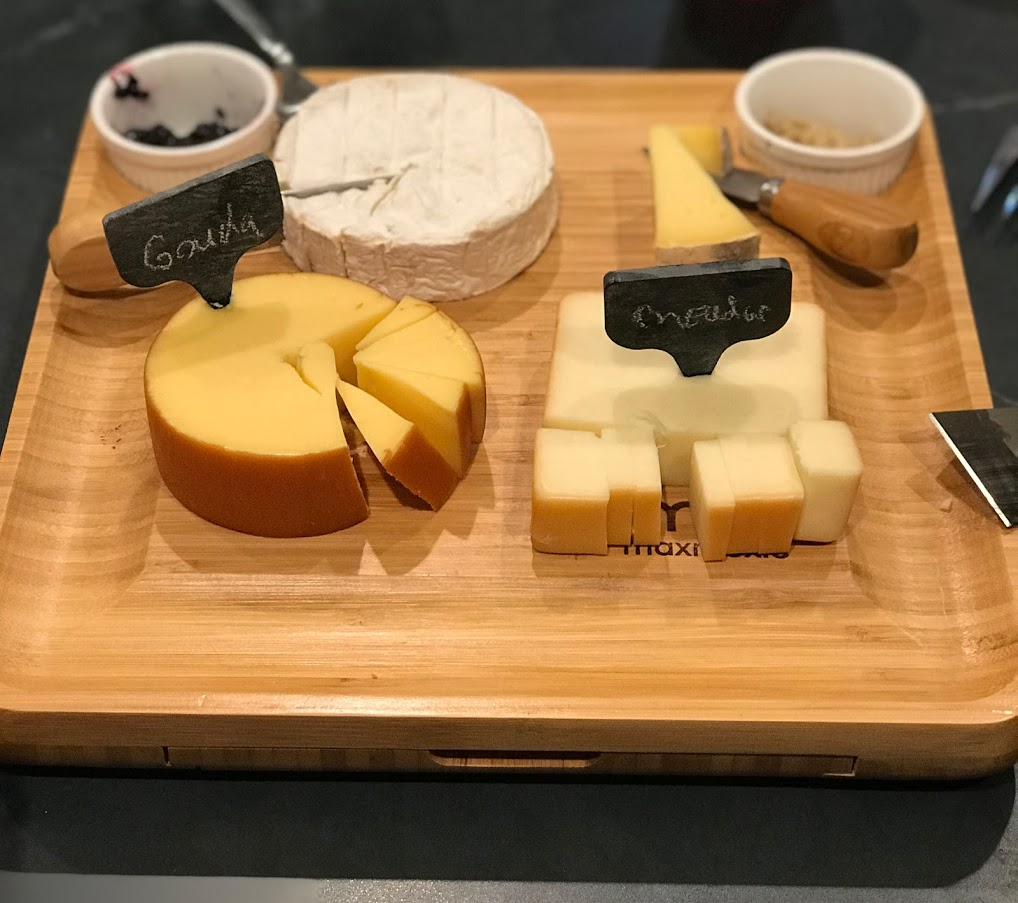
\includegraphics[width=6in]{images/IMG_0506.jpg}
\nbvspace[3]
\normalsize

%DOHA\\
%\large
%PUBLISHED IN THE WILD
\nbvspace[1]
\end{center}
\end{titlepage}

\clearpage\null\vfill
\pagestyle{empty}
\begin{minipage}[b]{0.9\textwidth}
\footnotesize\raggedright
\setlength{\parskip}{0.5\baselineskip}
Copyright \copyright 2019--\the\year\ Steven Hickson\par
Permission is granted to copy, distribute and\slash or modify 
the template of this document but not the contents or recipes. 
\end{minipage}
\vspace*{2\baselineskip}
\cleardoublepage
\rfoot{\thepage}

%\pagestyle{headings}
% This sets up the header and adds the page number.
\pagestyle{fancy}
\fancyhead[R,L]{\leftmark\hspace*{\hfill}Page \thepage}
%\pagenumbering{arabic}
%\fancyfoot[R]{\thepage}

%\setcounter{tocdepth}{1}
\tableofcontents

% This adds the chapter to the top

\part{Breads and Breakfast}
\chapter{Breads}
\begin{figure}[h]
\begin{center}
   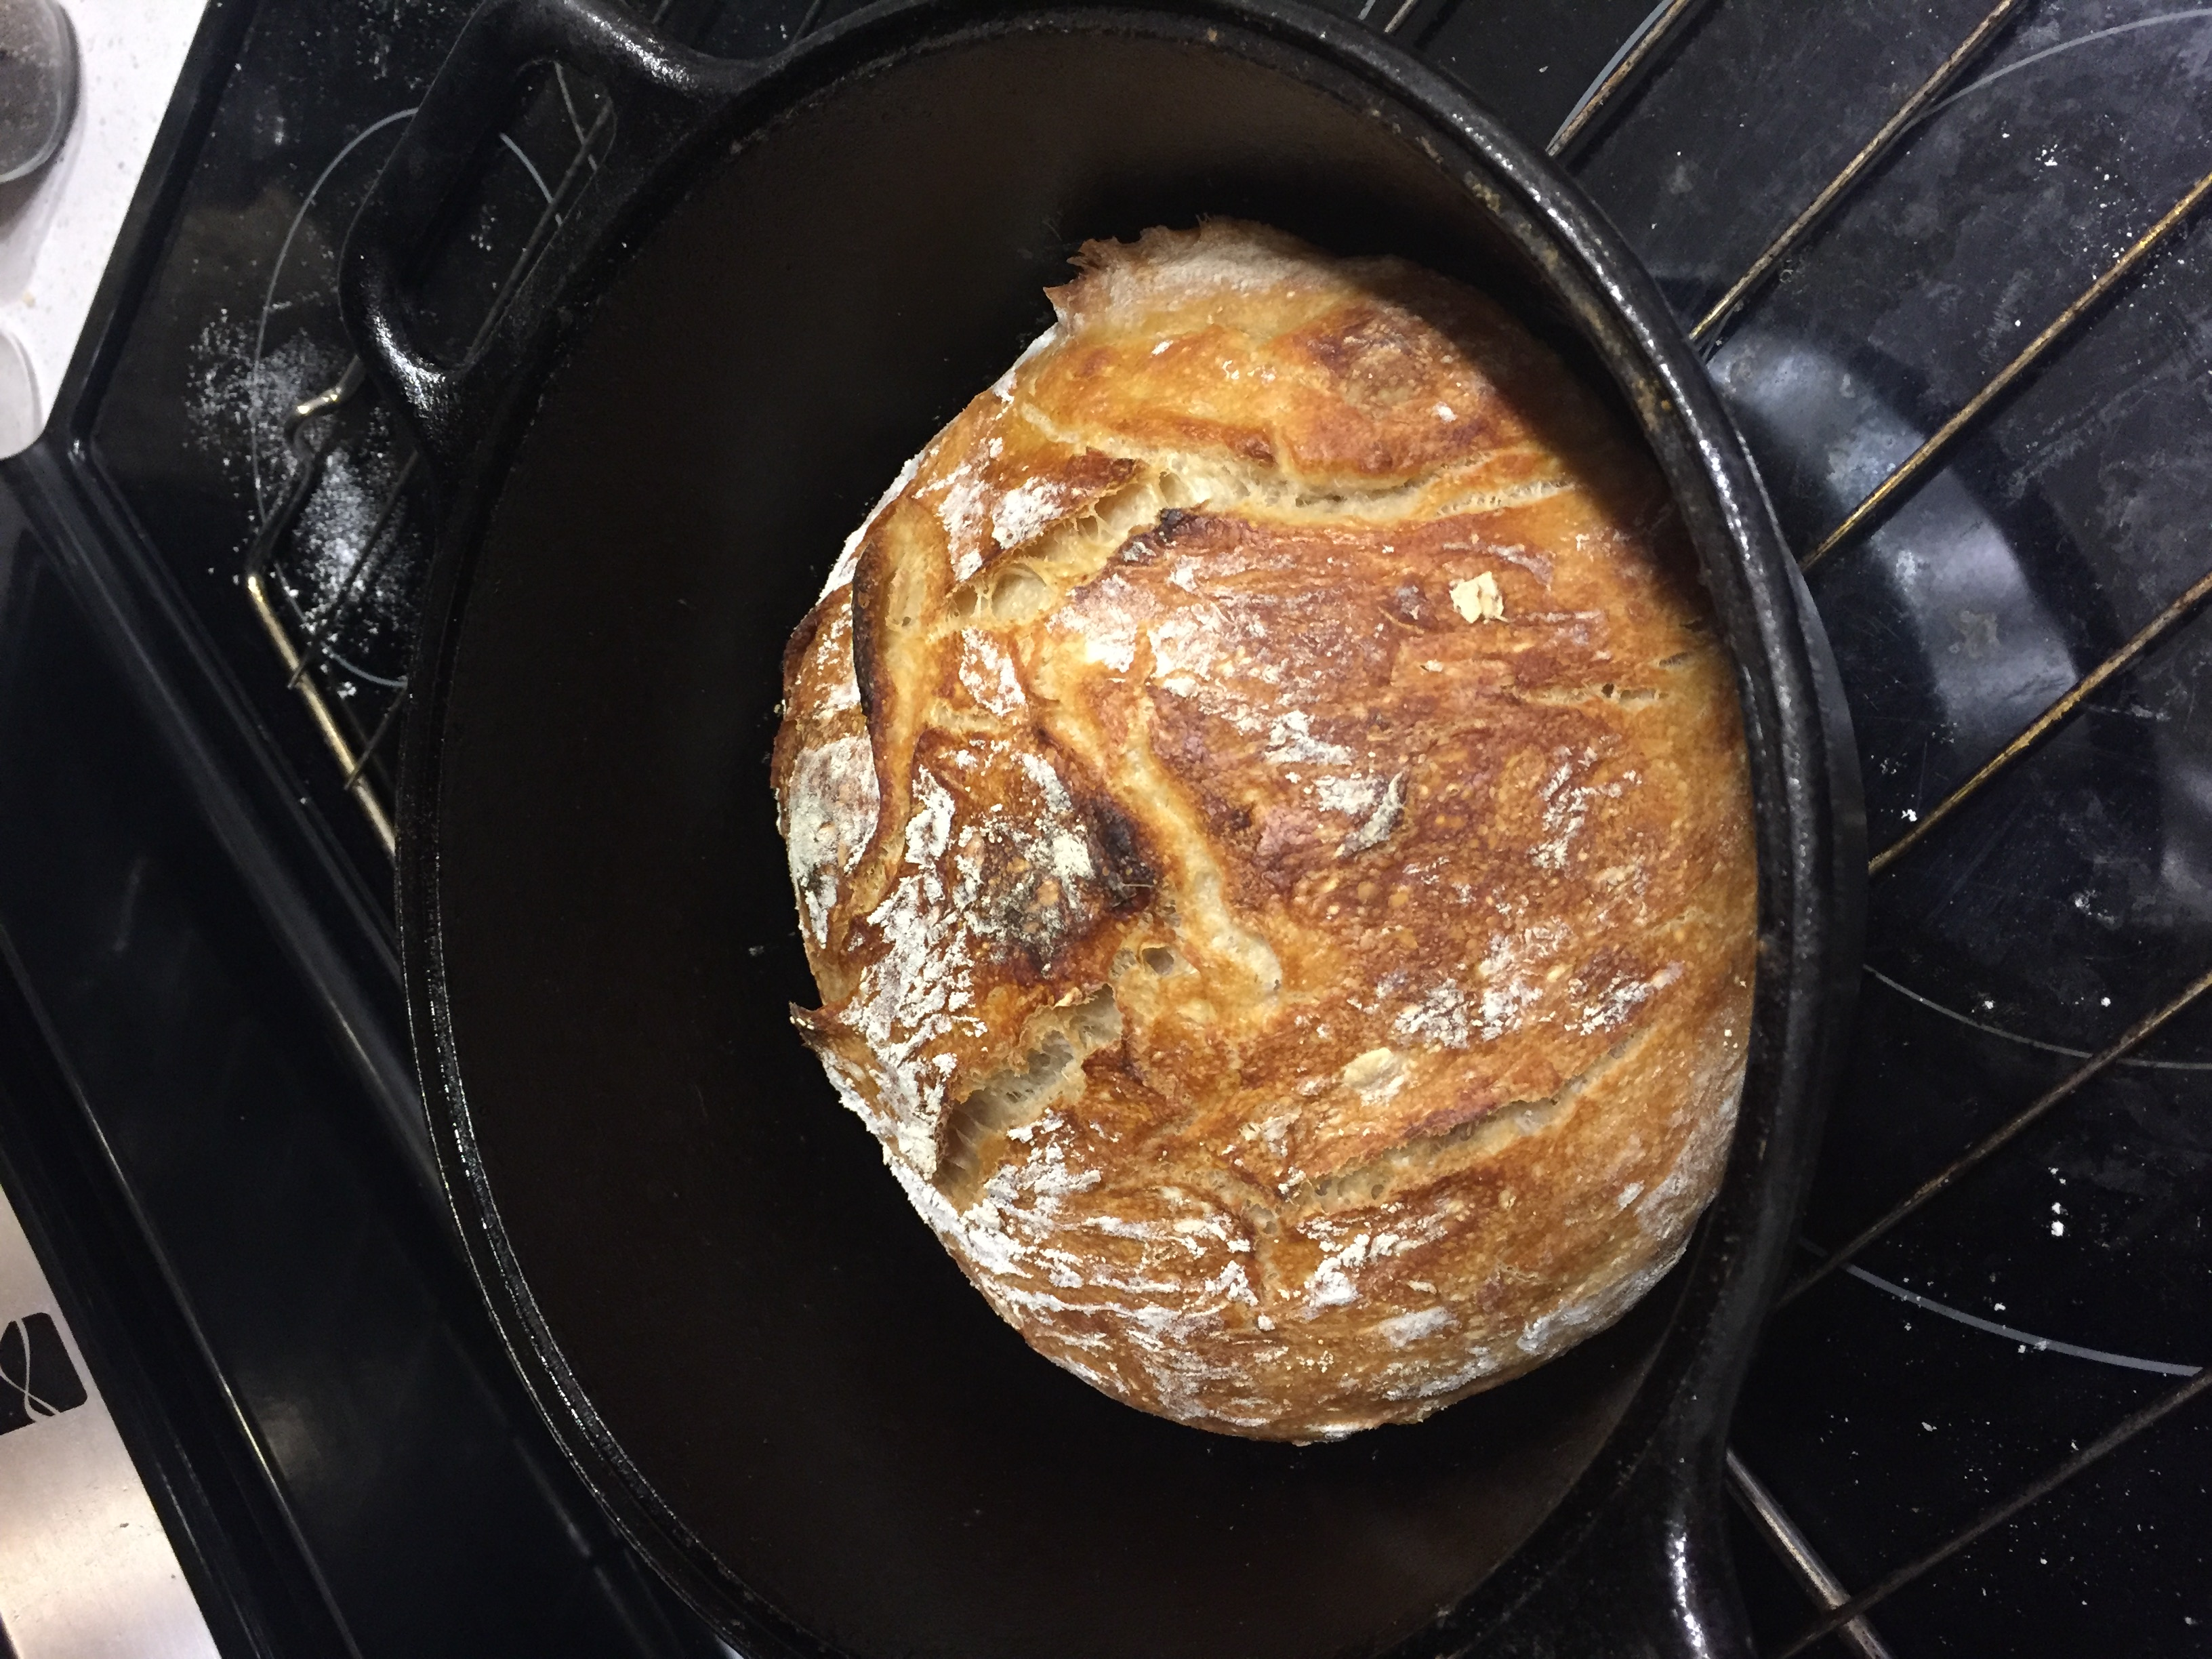
\includegraphics[width=0.9\linewidth, angle=270]{images/IMG_6927.JPG}
\end{center}
\end{figure}
\newpage

\newrecipe
\begin{recipe}
[
preparationtime = {\unit[3.5]{h}},
bakingtime = {\unit[30]{m}},
portion = {\portion{1}}
]
{Foccacia with Savory Olives}

\ingredients{
1 $\frac{1}{2}$ cups warm water\\ 
1 tablespoon sugar\\ 
2 (1/4 ounce) packages active dry yeast\\ 
3 $\frac{1}{2}$ cups all purpose flour\\ 
2 teaspoons kosher salt\\ 
6 tablespoons extra-virgin olive oil, divided\\ 
1/3 cup black olives, sliced\\ 
$\frac{1}{4}$ cup slivered or sliced almonds\\ 
2 tablespoons chopped fresh savory\\ 
Coarse sea salt and freshly ground pepper
}

\preparation{
\step In a small bowl, dissolve the sugar in the warm water. Sprinkle the yeast over the water and let stand for 10 minutes.
\step In the bowl of a mixer fitted with a paddle attachment, add 3 cups of the
flour, the salt, 2 tablespoons of the olive oil and the yeast mixture. 
\step Turn the mixer on low speed and slowly mix until the dough comes together. 
\step Gradually add remaining flour. If the dough seems too wet, add up to $\frac{1}{4}$ cup more flour. 
\step Place the dough into an oiled bowl, cover and let rise in a warm place, free from drafts for 3 hours.
\step Preheat the oven to 375 degrees.\\ 
\step Punch down the dough and transfer onto a lightly greased 9 by 13 inch baking sheet. Spread the dough to the edges of the baking sheet. Using your fingertips make dimples in the dough.
\step Drizzle the dough with the 2 tablespoons of the olive oil and sprinkle with the olives, almonds and savory.
\step Sprinkle lightly with salt and pepper. Then, bake for 30 to 35 minutes or until golden brown.
\step Drizzle with remaining 2 tablespoons of high quality olive oil.
}
\end{recipe}
\newrecipe
\begin{recipe}
[
preparationtime = {\unit[1.5]{h}},
portion = {\portion{2}},
source = Bobby Flay
]
{Pizza Dough}\label{pg:pizza_dough}

\hint{Using bread flour will give you a much crisper crust. If you can't find bread flour, you can substitute it with all-purpose flour which will give you a chewier crust.}

\ingredients{
3 1/2 to 4 cups bread flour\\ 
extra flour for rolling\\ 
1 teaspoon sugar\\ 
1 envelope instant dry yeast\\ 
2 teaspoons kosher salt\\ 
1 1/2 cups water, 110\degree F\\ 
2 tablespoons olive oil, plus 2 teaspoons\\ 
}

\preparation{
\step Combine the bread flour, sugar, yeast and kosher salt in the bowl of a stand mixer and combine. 
\step While the mixer is running, add the water and 2 tablespoons of the oil and beat until the dough forms into a ball. If the dough is sticky, add additional flour, 1 tablespoon at a time, until the dough comes together in a solid ball. If the dough is too dry, add additional water, 1 tablespoon at a time.
\step Scrape the dough onto a lightly floured surface and gently knead into a smooth, firm ball.
\step Grease a large bowl with the remaining 2 teaspoons olive oil, add the dough, cover the bowl with plastic wrap and put it in a warm area to let it double in size, about 1 hour. 
\step Turn the dough out onto a lightly floured surface and divide it into 2 equal pieces. Cover each with a clean kitchen towel or plastic wrap and let them rest for 10 minutes.
}
\end{recipe}



\chapter{Breakfast}
\begin{figure}[h]
\begin{center}
   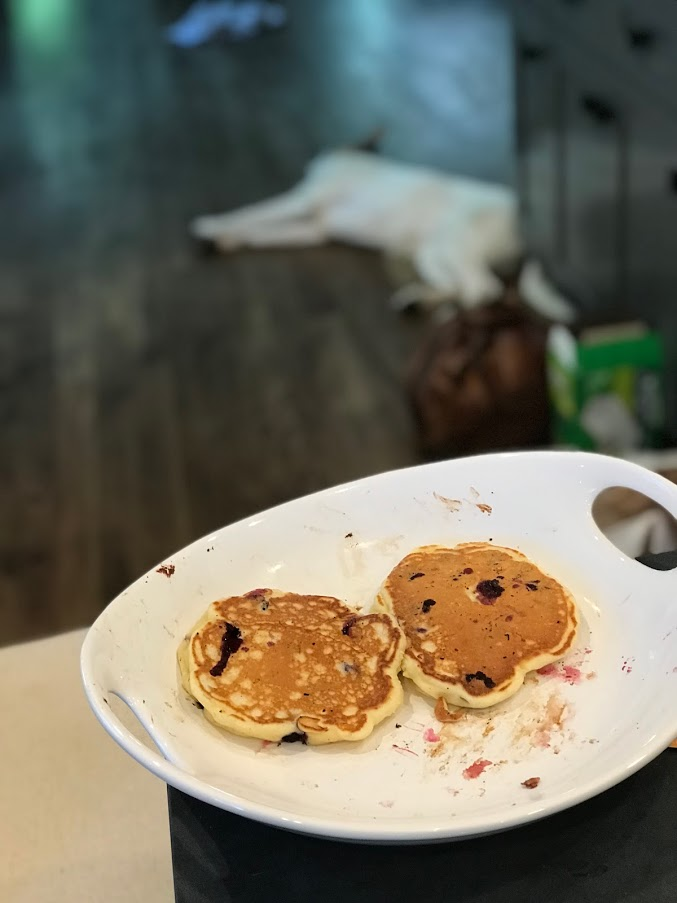
\includegraphics[width=0.65\linewidth]{images/IMG_2540.jpg}
\end{center}
\end{figure}
\newpage
\newrecipe
\begin{recipe}
[
preparationtime = {\unit[1]{h}},
portion = {\portion{4-6}},
source = Paula Dean
]
{Baked French Toast Casserole with Maple Syrup}

\ingredients{
1 loaf French bread (13-16 ounces)\\ 
8 large eggs\\ 
2 cups half and half\\ 
1 cup milk\\ 
2 tablespoons granulated sugar\\ 
1 teaspoon vanilla extract\\ 
$\frac{1}{4}$ teaspoon ground cinnamon\\ 
$\frac{1}{4}$ teaspoon ground nutmeg\\ 
Dash salt\\ 
Maple Syrup\\ 
\\ 
\textbf{Praline Topping}:\hspace*{\fill} \\ 
2 sticks butter\\ 
1 cup packed brown sugar\\ 
1 cup chopped pecans\\ 
2 tablespoons light corn syrup\\ 
$\frac{1}{2}$ teaspoon ground cinnamon\\ 
$\frac{1}{2}$ teaspoon ground nutmeg\\ 
}

\preparation{
\step Slice French bread into 20 slices, 1 inch each. Arrange slices in a generously buttered 9 by 13 inch flat baking dish in 2 rows, overlapping the slices. 
\step In a large bowl, combine the eggs, half and half, milk, sugar, vanilla, cinnamon, nutmeg and salt and beat with a rotary beater or whisk until blended but not too bubbly. 
\step Pour mixture over the bread slices, making sure all are covered evenly with the milk-egg mixture. Spoon some of the mixture between the slices.
\step If prepping, Cover with foil and refrigerate whenever you are ready (overnight works well).
\step When ready to make, preheat the oven to 350 degrees.
\step For the praline topping, combine all the ingredients in a medium bowl and blend well.
\step Spread the praline topping evenly over the bread and bake for 40 minutes until puffed and lightly golden.
\step Serve with maple syrup.
}
\end{recipe}
\newrecipe
\begin{recipe}
[
preparationtime = {\unit[20]{m}},
portion = {\portion{4-5}},
]
{Buttermilk Pancakes}

\ingredients{
1-$\frac{1}{2}$ cups all-purpose flour\\ 
$\frac{1}{2}$ cup whole-wheat flour\\ 
1 tsp cream of tartar\\ 
1 tsp baking soda\\ 
$\frac{1}{2}$ tsp. salt\\ 
$\frac{1}{2}$ tsp. pumpkin pie spice\\ 
2 large eggs\\ 
1-$\frac{3}{4}$ cups buttermilk\\ 
2 tsp. sugar\\ 
4 tablespoons butter, melted\\ 
}

\hint{Add blueberries, chocolate chips, or other fruit to your liking in step 3.}

\preparation{
\step Whisk the all-purpose flour, whole wheat flour, cream of tartar, baking soda, pumpkin pie spice and salt in a medium bowl.
\step Whisk the eggs, buttermilk, and sugar in a large bowl until foamy, then stir in the melted butter. 
\step Add the flour mixture and stir until just combined. (The batter will be thick and okay if there is a few lumps)
\step Heat a large skillet over medium heat until hot. Brush lightly with vegetable oil.
\step Drop a heaping $\frac{1}{4}$ cup of batter into the skillet for each pancake (you can spread it out with the back of a spoon).
\step Cook until the bubbles on top burst and the edges until golden brown; about 4 minutes without being disturbed.
\step Flip and cook until golden brown 2 to 3 minutes.\\ 
\step Serve with butter and syrup.
}
\end{recipe}

\part{Desserts and Drinks}

\chapter{Desserts}
\begin{figure}[h]
\begin{center}
   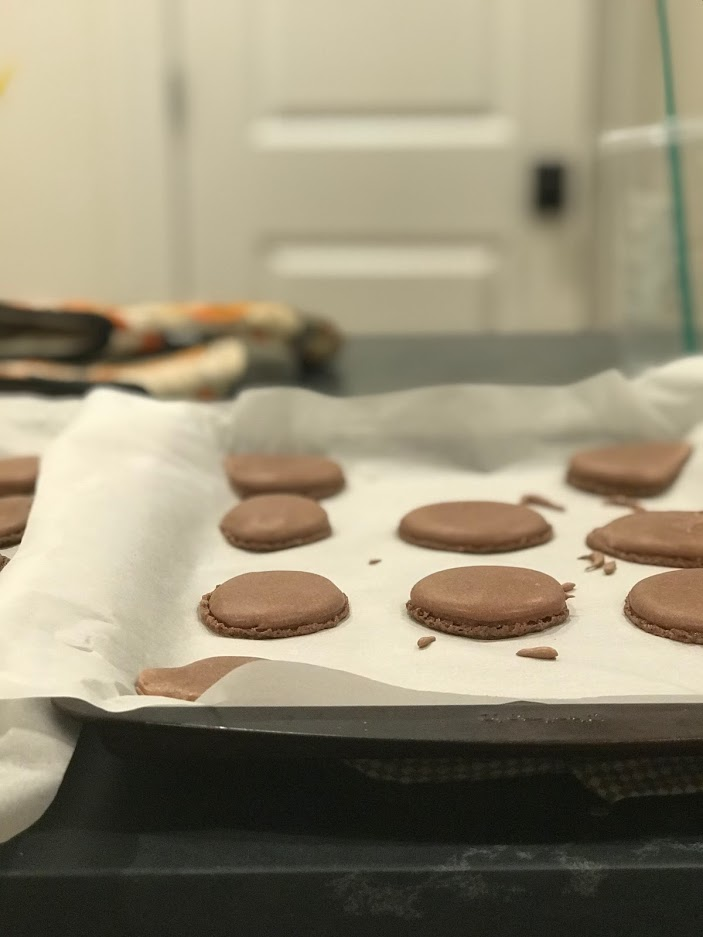
\includegraphics[width=0.65\linewidth]{images/IMG_2198.jpg}
\end{center}
\end{figure}
\newpage

\newrecipe
\begin{recipe}
[
preparationtime = {\unit[30]{m}},
bakingtime = {\unit[30]{m}},
portion = {\portion{4-6}},
source = Mom's blue ribbon recipe
]
{Apple Cheese Crisp}

\ingredients{
4 cups peeled, sliced apples\\ 
1 teaspoon water\\ 
$\frac{1}{2}$ teaspoon lemon juice\\ 
1 cup flour\\ 
$\frac{1}{2}$ cup brown sugar\\ 
2 tablespoons sugar\\ 
$\frac{1}{4}$ teaspoon cinnamon\\ 
$\frac{1}{4}$ teaspoon nutmeg\\ 
1 stick butter\\ 
1 cup shredded cheddar cheese\\ 
}

\preparation{
\step Sprinkle water and lemon juice over apples in baking dish or pie pan.
\step Combine flour, sugars, spices. Cut in butter until mixture is crumbly.
\step Add cheddar cheese and sprinkle over apples.\\ 
\step Bake 30 minutes at 350 degrees. Serve warm topped with ice cream or whipped cream
}
\end{recipe}
\newrecipe
\begin{recipe}
[
preparationtime = {\unit[1]{h}},
bakingtime = {\unit[40]{m}},
portion = {\portion{4-6}}
]
{Apple-Oatmeal Crisp with Irish Whiskey Cream}

\ingredients{
1 stick cold unsalted butter (in pieces)\\ 
2 pounds Rome apples\\ 
2 tablespoons fresh lemon juice\\ 
1 cup packed light brown sugar\\ 
1 cup all purpose flour\\ 
2 tablespoons Irish Whiskey\\ 
1 teaspoons cinnamon\\ 
$\frac{1}{4}$ teaspoon cardamom\\ 
Pinch salt\\ 
$\frac{1}{4}$ cup Irish oatmeal\\ 
$\frac{1}{4}$ cup toasted, chipped walnut pieces\\ 
\\ 
\textbf{Irish Whiskey Cream:}\hspace*{\fill}\\ 
1 cup heavy cream\\ 
1 tablespoon sugar\\ 
2 tablespoons Irish whiskey\\ 
}

\preparation{
\step Peal, core, and slice the apples.\\ 
\step Preheat the oven to 375 degrees. Lightly butter an 11 by 7 inch baking pan and set aside.
\step In a large skillet, melt 3 tablespoons of butter over medium-high heat.
\step Add the apples, lemon juice, $\frac{1}{2}$ cup of the brown sugar and 1 tablespoon of the flour to the butter. Stir well and cook for 5 minutes.
\step Add the whiskey, cinnamon, cardamom and salt to the mixture, stir well and cook for 1 minute. Remove from the heat.
\step In a large bowl combine the remaining flour, oatmeal and remaining $\frac{1}{2}$ cup sugar.
\step Add the remaining 5 tablespoons of butter and mix well.
\step Put mixture in pan and bake about 35 to 40 minutes until crisp is golden.
\step Whip the cream until it begins to form soft peaks. Then, add the sugar and whiskey and beat until stiff peaks form.
\step Cover and chill the cream then seat hot with the Irish Whiskey cream.
}
\end{recipe}
\newrecipe
\begin{recipe}
[
preparationtime = {\unit[1]{h}},
bakingtime = {\unit[45]{m}},
portion = {\portion{3-5}},
source = Tyler Florence
]
{Bourbon Peach Cobbler}

\ingredients{
8 peaches\\ 
$\frac{1}{4}$ cup bourbon\\ 
$\frac{3}{4}$ cup sugar, plus more for dusting\\ 
2 tablespoons corn starch\\ 
1 teaspoon ground cinnamon\\ 
1-1/2 cups all purpose flour\\ 
2 teaspoons baking powder\\ 
$\frac{1}{2}$ teaspoon kosher salt\\ 
16 tablespoons (2 sticks) cold unsalted butter\\ 
$\frac{3}{4}$ cup heavy cream, plus more for brushing\\ 
}

\preparation{
\step Heat the oven to 375 degrees. Then, peel and slice the peaches to make 6-8 cups.\\ 
\step In a large bowl add the peaches, bourbon, $\frac{1}{4}$ cup sugar, cornstarch and cinnamon and mix well to coat the peaches evenly; set aside.
\step Prepare the dumplings: Into a bowl sift together the flour, $\frac{1}{2}$ cup sugar, baking powder and salt.
\step Cut 12 tablespoons (1-1/2 sticks) butter into small pieces. Add it to the flour mixture and cut it in with a pastry blender or your hands until the mixture looks like coarse bread crumbs. \step Pour in the cream and mix just until the dough comes together. Don't overwork the dough; it should be slightly sticky but manageable.
\step In a 10 inch cast iron skillet over medium low heat, melt the remaining 4 tablespoons butter. 
\step Add the peaches and cook gently until heated through about 5 minutes.\\ 
\step Drop the dough by  tablespoonfuls over the warm peaches. There can be gaps, the dough will puff up and spread out as it bakes.
\step Brush the top with some heavy cream and sprinkle with some sugar; put it into the oven on a baking sheet to catch any drips. 
\step Cook for 40 to 45 minutes until the top is browned and the fruit is bubbling.
}
\end{recipe}
\newrecipe
\begin{recipe}
[
preparationtime = {\unit[1.2]{h}},
bakingtime = {\unit[1]{h}},
portion = {\portion{3-4}},
source = Tyler Florence
]
{Cheesecake}

\ingredients{
\textbf{Graham Crust:}\hspace*{\fill}\\ 
1 $\frac{1}{2}$ cups graham cracker crumbs\\ 
5 tablespoons unsalted butter\\ 
$\frac{1}{3}$ cup firmly packed brown sugar\\ 
Pinch ground cinnamon\\ 
\textbf{Cheesecake Batter:}\hspace*{\fill}\\ 
2 pounds cream cheese, softened\\ 
1 $\frac{1}{3}$ cups sugar\\ 
5 large eggs\\ 
2 teaspoons vanilla\\ 
1 tablespoon lemon juice\\ 
$\frac{1}{4}$ teaspoon almond extract\\ 
$\frac{3}{4}$ cup sour cream\\ 
$\frac{3}{4}$ cup whipped cream\\ 
}

\preparation{
\step Preheat oven to 325 degrees.\\ 
\step For Graham crust: toss graham cracker crumbs, butter, brown sugar and cinnamon together in bottom of 9 inch springform pan and press firmly into pan bottom.
\step In a mixer bowl, blend cream cheese with sugar until well blended.
\step Add eggs and next 5 ingredients and blend well, stir on low speed about 5 minutes until totally smooth.
\step Pour into springform pan and place in oven. Bake until just set, about 60 to 75 minutes.
\step Turn of the oven, open door and let cool in oven 1 hour before refrigerating 8 hours or preferably overnight.
\step Serve with desired topping.
}
\end{recipe}
\newrecipe
\begin{recipe}
[
preparationtime = {\unit[40]{m}},
bakingtime = {\unit[30]{m}},
portion = {\portion{4-5}}
]
{Chocolate Chip Pie}

\ingredients{
\textbf{Pie:}\hspace*{\fill}\\ 
2 $\frac{3}{4}$ cups all purpose flour\\ 
1 $\frac{1}{2}$ teaspoons salt\\ 
1 teaspoon baking soda\\ 
1 $\frac{1}{4}$ teaspoons baking powder\\ 
1 cup (2 sticks) unsalted butter, softened\\ 
1 $\frac{1}{2}$ cups packed brown sugar\\ 
$\frac{1}{2}$ cup granulated sugar\\ 
3 large eggs\\ 
1 tablespoon vanilla extract\\ 
3 cups semisweet chocolate chips\\ 
2 cups chopped walnuts, optional\\ 
\textbf{Whipped cream:}\hspace*{\fill}\\ 
2 pints (4 cups) heavy cream\\ 
$\frac{1}{4}$ cup confectioners sugar\\ 
$\frac{1}{4}$ cup miniature semisweet chocolate chips\\ 
}

\preparation{
\step Preheat oven to 350 degrees. Grease 2 (9 inch) pie plates; set aside.
\step In a large bowl, sift together the flour, salt, baking soda and baking powder.
\step In the bowl of an electric mixer, cream together butter, brown sugar and granulated sugar.
\step Add the eggs, 1 at a time, beating until incorporated. Then beat in the vanilla.
\step Add flour mixture a little at a time and mix until fully combined.
\step Fold in the 3 cups chocolate chips and if desired the walnuts.
\step Divide the dough between the prepared pie plates and smooth the tops with a spatula.
\step Bake about 30 minutes or until pies are golden and slightly firm to the touch but still soft.
\step If the pies begin to darken too much before they are based through, over with foil and continue baking.
\step Let pies cool completely on a wire rack. While the pies cool, whip the cream and confectioners sugar until soft peaks form (tips curl).
\step Fold in the chocolate chips.\\ 
\step Refrigerate whipped cream until ready to use.\\ 
\step Spread the whipped cream over the pies and serve.\\ 
}
\end{recipe}
\newrecipe
\begin{recipe}
[
preparationtime = {\unit[1]{m}},
bakingtime = {\unit[15]{m}},
portion = {\portion{5-8}},
]
{Chocolate Marshmallow Pie}

\ingredients{
\textbf{For the crust:}\hspace*{\hfill}\\ 
12 whole chocolate graham crackers\\ 
%, roughly broken
3 tablespoons granulated sugar\\ 
1 stick unsalted butter, melted\\ 
\textbf{For the filling:}\hspace*{\hfill}\\ 
1 stick unsalted butter\\ 
8 oz. milk chocolate, chopped\\ 
$\frac{1}{2}$ cup granulated sugar\\ 
2 large eggs\\ 
2 tsp. Vanilla extract\\ 
$\frac{1}{2}$ tsp. salt\\ 
$\frac{1}{2}$ cup flour\\ 
\textbf{For the topping:}\hspace*{\hfill}\\ 
1 cup cold heavy cream\\ 
$\frac{2}{3}$ cup marshmallow cream\\ 
1 tbsp. confectioners sugar\\ 
Shaved chocolate for topping\\ 
}

\preparation{
\step Preheat the oven to 350 degrees. Roughly break up the graham crackers.\\ 
\\ \textbf{Make the crust:}
\step Pulse the graham crackers and granulated sugar in a food processor until finely ground.
\step Add the melted butter and pulse a few times until combined. Press the mixture into the bottom and up the side of a 9 inch pie plate, making a thicker rim around the edge.
\step Bake until the top edge is firm and the bottom is dry about 15 minutes. Transfer to a rack and let cool completely.\\ 
\\ \textbf{Make the filling:}
\step Melt the butter and chocolate in a medium saucepan over medium heat, stirring occasionally until smooth.
\step Transfer to a medium bowl and let mixture cool 5 minutes.
\step Whisk in the granulated sugar, eggs, vanilla and salt until smooth.\\ 
\step Whisk in the flour until combined. Then, pour the filling into the cooled crust.\\ 
\step Bake until the filling is set and a toothpick inserted into the center comes out clean, 35 to 40 minutes.
\step Transfer to a rack and let cool completely.\\ 
\\ \\ \textbf{Make the topping.}
\step Combine the heavy cream, marshmallow cream and confectioners sugar in a food processor and pulse, scraping down the processor until the mixture is thick.
\step Spoon the topping onto the center of the pie. Top with shaved chocolate.
}
\end{recipe}
\newrecipe
\begin{recipe}
[
preparationtime = {\unit[2.5]{h}},
portion = {\portion{3}}
]
{Chocolate Mousse}

\ingredients{
3 eggs, separated\\ 
1 $\frac{1}{2}$ teaspoon vanilla\\ 
$\frac{1}{2}$ teaspoon almond extract\\ 
4 (1 ounce) squares semisweet chocolate\\ 
$\frac{1}{2}$ teaspoon cream of tarter\\ 
$\frac{1}{2}$ cup sugar\\ 
1 cup whipping cream\\ 
}

\preparation{
\step Melt chocolate with a double boiler and then cool slightly.
\step Make a meringue using steps 3-5.\\ 
\step Beat egg yolks, lightly add flavorings and chocolate to egg yolks, stirring well.
\step Beat egg whites (at room temperature) and cream of tarter at high speed of an electric mixer until frothy.
\step Gradually add sugar, 1 tablespoon at a time beating until stiff peaks form and sugar dissolves (2 to 4 minutes).
\step Stir about $\frac{1}{4}$ of the meringue into chocolate mixture. Then, fold remaining meringue into chocolate mixture.
\step Beat whipping cream at medium speed of an electric mixer until soft peaks form. Then, Fold cream into chocolate mixture.
\step Cover and chill at least 2 hours.
}
\end{recipe}
\newrecipe
\begin{recipe}[
preparationtime = {\unit[20]{m}},
bakingtime = {\unit[55]{m}},
portion = {\portion{4-5}}
]
{Chocolate Pecan Pie}

\ingredients{
$\frac{1}{2}$ (15 ounce) refrigerated piecrusts\\ 
1 $\frac{1}{2}$ cups chopped pecans\\ 
1 cup semisweet chocolate morsels\\ 
$\frac{1}{2}$ cup granulated sugar\\ 
$\frac{1}{2}$ cup firmly packed brown sugar\\ 
1 cup dark corn syrup\\ 
$\frac{1}{4}$ cup bourbon\\ 
4 large eggs\\ 
2 teaspoons cornmeal\\ 
$\frac{1}{2}$ teaspoon salt\\ 
$\frac{1}{4}$ cup butter\\ 
2 teaspoons vanilla\\ 
}\\ 

\preparation{
\step Fit piecrust into a 9 inch pieplate according to the package directions; fold edges under and crimp.
\step Sprinkle chopped pecans and chocolate morsels evenly onto piecrust; set aside.
\step Combine sugars, corn syrup, and bourbon in a large saucepan; bring to a boil over medium heat. Cook 3 minutes, stirring constantly.
\step Whisk together eggs and remaining ingredients (cornmeal, salt, butter, and vanilla). 
\step Gradually stir about $\frac{1}{4}$ hot mixture into egg mixture (slowly do this).
\step Add the remaining hot mixture, stirring constantly. Then, pour filling into piecrust.
\step Bake at 325 degrees for 55 minutes, cool.
}
\end{recipe}

\newrecipe
\begin{recipe}[
preparationtime = {\unit[4.5]{h}},
portion = {\portion{5-7}},
source = Mom's recipe
]
{Christmas Trifle}

\ingredients{
1 pound cake (any flavor)\\ 
\textbf{Filling:}\hspace*{\fill}\\ 
1 quart milk\\ 
2 cups sugar\\ 
1 teaspoon vanilla\\ 
10 large egg yolks, beaten\\ 
$\frac{1}{2}$ cup cornstarch (dissolved in water)\\ 
$\frac{1}{2}$ cup water\\ 
2 tablespoons unsalted butter\\ 
\textbf{To assemble the trifle:}\hspace*{\fill}\\ 
1 quart heavy cream\\ 
$\frac{1}{4}$ cup sugar\\ 
1 cup orange flavored liqueur (Grand Marnier)\\ 
4-6 pints fresh raspberries\\ 
}

\preparation{
\\ \textbf{Filling:} 
\step Combine the milk, sugar and vanilla in a large heavy bottomed saucepan over medium-high heat. Whisk to dissolve the sugar.
\step When the mixture comes to a simmer after 5 minutes, take 1 cup of the milk and sugar mixture and add it to the yolks. Whisk to blend well.
\step Slowly add the yolks to the milk and sugar mixture in the saucepan, whisking constantly. \step Cook over medium heat until it thickens slightly, 4 to 5 minutes, whisking occasionally.
\step Over medium heat, slowly add this mixture to the saucepan, whisking constantly for 1 minute. Using a wooden spoon, continue stirring for about 2 minutes.
\step Add the butter and stir until it is completely melted and the mixture has thickened to a custard, about 2 minutes.
\step Pour the mixture into a glass bowl. Cover with plastic wrap, pressing the wrap down on the surface of the custard to prevent a skin from forming.
\step Cool completely and chill for at least 4 hours.\\ \\ 
\\ \textbf{To assemble the trifle:}
\step Cut the cake into 1 inch cubed size pieces.\\ 
\step Beat the cream with an electric mixer on high speed for about 2 minutes.\\ 
\step Add the sugar and beat until a mixture is thick and forms soft peaks, 1 to 2 minutes. Set aside.
\step Beat the custard with a wire whisk until it is smooth. Set aside.\\ 
\step Spread out the cubed pound cake evenly on a piece of parchment paper. Drizzle the orange liqueur over the pound cake.
\step Spread 1 cup of the cream filling on the bottom of a large, deep glass trifle bowl. Top with a layer of pound cake.
\step Arrange raspberries on top of the pound cake. Then, spread 2 cups of the cream on top of the raspberries. Top with more pound cake, then raspberries.
\step Spread another cup of the cream and top with the remaining pound cake and raspberries. Then, spread the remaining cream on top of the raspberries.
\step Mound the whipped cream evening over the top.\\ 
\step Serve immediately or keep chilled until ready to serve.
}
\end{recipe}

\newrecipe
\begin{recipe}[
preparationtime = {\unit[20]{m}},
bakingtime = {\unit[1.5]{h}},
portion = {\portion{4-5}}
]
{Classic Pound Cake}

\ingredients{
4 cups all purpose flour\\ 
3 cups sugar\\ 
2 cups butter, softened\\ 
$\frac{3}{4}$ cup milk\\ 
6 large eggs\\ 
2 teaspoons vanilla extract\\ 
}

\preparation{
\step Preheat oven to 325 degrees.\\ 
\step Place flour, sugar, butter, milk, eggs and vanilla (in that order) in a 4 quart bowl of a heavy duty electric stand mixer.
\step Beat at low speed 1 minute, stopping to scrape down sides.
\step Beat at medium speed 2 minutes.\\ 
\step Pour unto a greased and floured 10 inch tube pan and smooth.\\ 
\step Bake for 1 hour and 30 minutes or until a long wooden pick inserted in center comes out clean.
\step Cool in plan on a wire rack 10 minutes. Remove from pan to wire rack and cool completely (about 1 hour).
}
\end{recipe}

\newrecipe
\begin{recipe}[
preparationtime = {\unit[10]{m}},
bakingtime = {\unit[1]{h}},
portion = {\portion{3-4}}
]
{Coffee Cake}

\ingredients{
1 box yellow cake mix\\ 
1 package instant butterscotch pudding\\ 
4 eggs\\ 
$\frac{1}{2}$ cup oil\\ 
1 cup sour cream\\ 
}

\preparation{
\step Grease a tube pan with butter. Preheat oven 350 degrees.
\step Mix ingredients for 7 minutes.\\ 
\step Stir $\frac{1}{2}$ cup sugar, 2 teaspoons cinnamon and 1/3 cup nuts. Sprinkle sugar mixture on bottom of pan.
\step Spoon batter alternating the sugar mixture.\\ 
\step Bake 55-60 minutes. Cool upright in pan.
}
\end{recipe}

\newrecipe
\begin{recipe}[
preparationtime = {\unit[10]{m}},
portion = {\portion{3-4}}
]
{Cream Cheese Frosting}

\ingredients{
4 tablespoons butter, room temperature\\ 
4 ounces cream cheese, room temperature\\ 
3 cups confectionery sugar, sifted\\ 
1 teaspoon vanilla\\ 
1 tablespoon milk\\ 
}

\preparation{
\step Cream butter \& cream cheese, add sugar about $\frac{1}{2}$ cup at a time.
\step Add vanilla and milk.
}
\end{recipe}

\newrecipe
\begin{recipe}[
preparationtime = {\unit[30]{m}},
bakingtime = {\unit[1]{h}},
portion = {\portion{4-5}}
]
{Eggnog pound cake}

\ingredients{
1 $\frac{3}{4}$ cups all-purpose flour\\ 
2 teaspoons baking powder\\ 
$\frac{1}{2}$ teaspoon salt\\ 
$\frac{1}{2}$ teaspoon ground nutmeg\\ 
$\frac{1}{2}$ teaspoon cinnamon\\ 
1 cup sugar\\ 
$\frac{1}{2}$ cup (1 stick) unsalted butter, softened\\ 
2 tablespoons dark rum\\ 
2 teaspoons vanilla\\ 
5 large egg yolks\\ 
$\frac{3}{4}$ cup milk\\ 
}

\preparation{
\step Preheat the oven to 350 degrees. Grease and flour a 9x5x3 inch loaf pan.
\step Combine the flour, baking powder, salt and spices in a small bowl.
\step Using an electric mixer on low speed, beat the sugar, butter, rum, vanilla, and egg yolks in a large bowl for 60 seconds, scraping the bowl frequently.
\step Increase the speed to high and beat for 5 minutes, scraping the bowl occasionally.
\step Reduce the speed to low and mix in one-third of the flour mixture, alternating with the milk until just combined.
\step Pour the batter into the prepared pan.\\ 
\step Bake for 50-60 minutes or until a toothpick inserted in the center comes out clean.\\ 
\step Cool in the pan for 10 minutes, then remove from the pan and cool completely.
}
\end{recipe}

\newrecipe
\begin{recipe}[
preparationtime = {\unit[20]{m}},
bakingtime = {\unit[40]{m}},
portion = {\portion{3-5}}
]
{French Chocolate Silk Pie}

\ingredients{
1 prebaked 9 inch pastry shell\\ 
4 tablespoons unsalted butter\\ 
1 cup coarsely chopped semisweet chocolate\\ 
1 (14 ounce) can sweetened condensed milk\\ 
$\frac{1}{2}$ cup half and half or light cream\\ 
Pinch of salt\\ 
2 large eggs\\ 
1 teaspoon vanilla\\ 
1 tablespoon flour\\ 
}

\preparation{
\step Preheat oven to 350 degrees.\\ 
\step In a saucepan melt butter and chocolate together over low heat.
\step In a medium bowl, whisk condensed milk with warm chocolate butter mixture.
\step Stir in cream, salt, eggs, vanilla and flour; whisk well to mix.
\step Spoon filling into baked crust and bake 35 to 40 minutes until edges of pie are lightly golden brown.
\step Serve warm or chilled with whipped cream, chocolate shavings, vanilla ice cream or hot fudge sauce.
}
\end{recipe}

\newrecipe
\begin{recipe}[
preparationtime = {\unit[15]{m}},
bakingtime = {\unit[30]{m}},
portion = {\portion{4-6}}
]
{Ginger Pear Crisp}

\ingredients{
6 pears, peeled and sliced\\ 
1 tablespoon finely chopped ginger\\ 
$\frac{1}{2}$ cup brown sugar\\ 
$\frac{1}{2}$ cup raisons\\ 
2 teaspoons cinnamon\\ 
2 tablespoons butter, cut into bits\\ 
\\ 
\textbf{Topping:}\hspace*{\hfill}\\ 
$\frac{1}{4}$ cup flour\\ 
$\frac{3}{4}$ cup rolled oats\\ 
$\frac{1}{4}$ cup brown sugar\\ 
$\frac{1}{4}$ cup sugar\\ 
1 teaspoon cinnamon\\ 
6 tablespoons butter\\ 
}

\preparation{
\step Preheat oven to 350 degrees. Toss first six ingredients together in a bowl and mix.
\step Pour into a buttered baking dish.\\ 
\step Using a fork combine the remaining six ingredients. Spoon topping across pears.
\step Bake for 30 minutes or until brown and bubbly.
}
\end{recipe}

\newrecipe
\begin{recipe}[
preparationtime = {\unit[20]{m}},
portion = {\portion{4-6}}
]
{Glazed Pineapple}

\ingredients{
4 tablespoons melted butter\\ 
$\frac{1}{4}$ cup brown sugar\\ 
$\frac{1}{4}$ teaspoon cinnamon\\ 
$\frac{1}{4}$ teaspoon vanilla extract\\ 
Pinch of salt\\ 
Splash of rum\\ 
}

\preparation{
\step Mix melted butter, brown sugar, cinnamon, vanilla extract and rum in a bowl.
\step Slice a pineapple in half lengthwise (keeping the top attached), then cut each half into 3 long wedges; cut out the core.
\step Place 2 wedges on a sheet of foil; brush with the spiced butter and fold up. Repeat to make 2 more packets.
\step Grill over medium heat until the pineapple is soft and golden on the bottom, 15 to 20  minutes.
}
\end{recipe}

\newrecipe
\begin{recipe}[
preparationtime = {\unit[6.5]{h}},
portion = {\portion{3-5}}
]
{Graham Banana Pudding}

\ingredients{
4 cups half \& half\\ 
4 large egg yolks\\ 
1 $\frac{1}{2}$ cups sugar\\ 
$\frac{1}{4}$ cup cornstarch\\ 
$\frac{1}{4}$ teaspoon salt\\ 
3 tablespoons butter\\ 
2 teaspoons vanilla extract\\ 
1 (5 ounce) package graham crackers, divided\\ 
4 large ripe bananas, sliced and divided\\ 
2 cups whipping cream\\ 
2 tablespoons sugar\\ 
}

\preparation{
\step Whisk together first 5 ingredients in a saucepan over low heat; cook whisking constantly 8 to 10 minutes or until thickened.
\step Remove from heat; stir in butter and vanilla.\\ 
\step Layer 5 graham crackers, half of bananas, and half of pudding in a 13x9 inch dish. Repeat layers.
\step Cover pudding and chill 6 hours.\\ 
\step Beat whipping cream and 2 tablespoons sugar at medium speed with an electric mixer until soft peaks form. Spread over pudding.
\step Chill until ready to serve.
}
\end{recipe}

\newrecipe
\begin{recipe}[
preparationtime = {\unit[10]{m}},
portion = {\portion{3-4}}
]
{Grandma's Doughnut Drops}

\ingredients{
2 cups flour\\ 
1/3 cup sugar\\ 
3 teaspoons baking powder\\ 
1 teaspoon salt\\ 
1 teaspoon nutmeg\\ 
1 egg lightly beaten\\ 
$\frac{3}{4}$ cup milk\\ 
3 tablespoons oil\\ 
Oil for fryer\\ 
}

\preparation{
\step Sift dry ingredients together.\\ 
\step Add egg, milk, oil and stir until smooth.\\ 
\step Drop dough by teaspoonful into hot oil.\\ 
\step Shake in cinnamon and sugar while warm.
}
\end{recipe}

\newrecipe
\begin{recipe}[
preparationtime = {\unit[30]{m}},
bakingtime = {\unit[55]{m}},
portion = {\portion{3-5}},
source = Emeril
]
{Honey Spice Cake with Rum Glaze}

\ingredients{
2 and 1/3 cups sifted cake flour\\ 
1 $\frac{1}{2}$ teaspoons baking powder\\ 
$\frac{1}{2}$ teaspoon baking soda\\ 
1 teaspoon ground ginger\\ 
1 teaspoon ground cinnamon\\ 
$\frac{1}{2}$ teaspoon ground cloves\\ 
$\frac{1}{2}$ teaspoon salt\\ 
1 $\frac{1}{2}$ sticks unsalted butter\\ 
2/3 cup real honey\\ 
$\frac{1}{2}$ cup sugar\\ 
3 large egg yolks\\ 
$\frac{3}{4}$ cup plus 2 tablespoons plain yogurt\\ 
4 large egg whites\\ 
1 $\frac{1}{4}$ cups sifted powdered sugar\\ 
1 $\frac{1}{2}$ teaspoons rum\\ 
}

\preparation{
\step Preheat oven to 350 degrees. Grease and flour 1 tube or bundt pan.
\step Sift the cake flour, baking power, baking soda, ginger, cinnamon, cloves and salt together, then sift again into a large bowl.
\step In another large bowl, beat the butter with an electric mixer on high speed until creamy.
\step Gradually add the honey and $\frac{1}{4}$ cup of the sugar to the butter and beat on high speed until well mixed, 2 to 4 minutes.
\step Beat in the egg yolks, 1 at a time. Beat on low and add the flour mixture in 3 parts, alternating with the yogurt in 2 parts.
\step Beat until smooth, scraping down the side of the bowl as necessary.
\step In another large bowl, beat the egg whites until soft peaks form.
\step Gradually add the remaining $\frac{1}{4}$ cup sugar, beating on high speed, until stiff.\\ 
\step Fold the egg whites into the batter. Then, pour the batter into the prepared pan and bake until a tester comes up clean 40 to 55 minutes.
\step Let the cake cool in the pan on a wire rack for 10 minutes and then invert the cake onto the rack and allow to cool completely.
\step In a small bowl combine the powdered sugar and sum and still to combine. Mixture should be a stiff glaze. If the glaze is too thick, thin with a bit of milk.
\step Using a spoon, drizzle the glaze all over the cake in a radom pattern. Let the cake sit until the glaze has hardened. Then serve.
}
\end{recipe}

\newrecipe
\begin{recipe}[
preparationtime = {\unit[30]{m}},
bakingtime = {\unit[10]{m}},
portion = {\portion{4-6}}
]
{Peanut Butter Kisses}

\ingredients{
48 Hershey's Kisses\\ 
$\frac{1}{2}$ cup shortening\\ 
$\frac{3}{4}$ cup creamy peanut butter\\ 
1/3 cup sugar\\ 
1/3 cup packed light brown sugar\\ 
1 egg\\ 
2 tablespoons milk\\ 
1 teaspoon vanilla\\ 
1 $\frac{1}{2}$ cups all purpose flour\\ 
1 teaspoon baking soda\\ 
$\frac{1}{2}$ teaspoon salt\\ 
Granulated sugar\\ 
}

\preparation{
\step Heat oven to 375 degrees. Remove wrappers from chocolates.
\step Beat shortening and peanut butter in large bowl. Add 1/3 cup granulated sugar and brown sugar; beat until fluffy.
\step Add egg, milk and vanilla; beat well.\\ 
\step Stir together flour, baking soda and salt; gradually beat into mixture.
\step Shape dough into 1 inch balls. Roll in sugar, place on ungreased cookie sheet.
\step Bake 8 to 10 minutes or until lightly browned.\\ 
\step Immediately press a chocolate kiss into center of each cookie.
\step Remove from cookie sheet to wire rack. Cool completely.
}
\end{recipe}

\newrecipe
\begin{recipe}
[
preparationtime = {\unit[30]{m}},
bakingtime = {\unit[30]{m}},
portion = {\portion{3-4}}
]
{Pear Spice Muffins}

\ingredients{
2 cups all-purpose flour\\ 
1 cup quick rolling oats\\ 
1 cup firmly packed light brown sugar\\ 
1 tablespoon baking powder\\ 
$\frac{1}{2}$ teaspoon salt\\ 
$\frac{1}{2}$ cup (1 stick) unsalted butter\\ 
1 teaspoon ground cinnamon\\ 
$\frac{1}{2}$ teaspoon ground allspice\\ 
2 eggs, lightly beaten\\ 
1 cup milk\\ 
2 grated, peeled pears (1 cup)\\ 
}

\preparation{
\step Preheat oven to 375 degrees. Grease the cups of a 12 muffin pan or line with baking cups.
\step Combine the flour, oats, brown sugar, baking powder and salt in a mixing bowl.
\step Using a pastry blender or your fingers, cut in the butter until the mixture resembles coarse crumbs. Set aside $\frac{3}{4}$ cup for the topping.
\step Stir in the cinnamon and allspice into the reserved topping.
\step Stir together the eggs, milk and grated pear in a small bowl.
\step Add the remaining dry ingredients all at once, stirring until just moist.
\step Divide the batter evenly among 12 muffin cups, filling each cup two thirds full.\\ 
\step Sprinkle the topping evenly over the batter; pat down gently to make it stick.\\ 
\step Bake for 25 to 30 minutes or until the tops spring back when lightly touched.\\ 
\step Remove the muffins from the pan immediately and cool on a wire rack.
}
\end{recipe}

\newrecipe
\begin{recipe}
[
preparationtime = {\unit[1.5]{h}},
bakingtime = {\unit[40]{m}},
portion = {\portion{3-5}}
]
{Pineapple Upside Down Cake}

\ingredients{
2 pounds of fresh pineapple\\ 
2 $\frac{1}{2}$ cups sugar\\ 
1 teaspoon ground cinnamon\\ 
1 teaspoon grated nutmeg\\ 
1 $\frac{1}{2}$ sticks butter, softened\\ 
1 teaspoon baking powder\\ 
1 teaspoon baking soda\\ 
Pinch of salt\\ 
2 whole eggs\\ 
1 teaspoon vanilla\\ 
1 cup milk\\ 
2 $\frac{1}{4}$ cups flour\\ 
}

\preparation{
\step Peel, core, and cube the pineapple. Preheat oven 350 degrees. 
\step In a mixing bowl, toss the pineapple with 1 cup of sugar, $\frac{1}{2}$ teaspoon cinnamon and $\frac{1}{2}$ teaspoon nutmeg.
\step In a hot cast iron skillet, melt $\frac{1}{2}$ stick of butter. Then, caramelize the pineapple, about 3 to 5 minutes.
\step For the batter: In a mixing bowl, cream one cup of the butter and 1 $\frac{1}{2}$ cups of sugar.
\step Next, stir in the eggs one at a time.\\ 
\step Stir in the baking powder, baking soda, vanilla, $\frac{1}{2}$ teaspoon cinnamon, teaspoon nutmeg and milk.
\step Add the flour and mix well.\\ 
\step Pour the cake batter evenly over the pineapple.\\ 
\step Bake for about 40 minutes, or until the cake is golden brown and pulls away slightly from the edges of the skillet.
\step Cool for about 30 minutes, then invert over a large platter.
}
\end{recipe}

\newrecipe
\begin{recipe}
[
preparationtime = {\unit[1]{h}},
bakingtime = {\unit[1.25]{h}},
portion = {\portion{4-5}},
sourece = Emeril w/ Mom's changes
]
{Pumpkin Cheesecake with Bourbon Spiked Cream}

\ingredients{
\\ \textbf{Cake:}\hspace*{\hfill}\\ 
1 $\frac{1}{2}$ cups ginger snaps crushed into crumbs\\ 
1 cup ground pecan pieces\\ 
1 stick melted butter\\ 
2 lbs cream cheese, softened and cubed\\ 
1 cup light brown sugar\\ 
6 eggs\\ 
$\frac{1}{2}$ cup heavy cream\\ 
$\frac{1}{2}$ cup all purpose flour\\ 
Pinch salt\\ 
$\frac{1}{2}$ teaspoon cinnamon\\ 
1 teaspoon vanilla\\ 
2 cups pumpkin puree\\ 
2 cups sweetened whipped cream\\ 
Dash bourbon\\ 
1 cup warm semisweet chocolate sauce\\ 
\textbf{Chocolate sauce:}\hspace*{\hfill}\\ 
$\frac{3}{4}$ cup half \& half\\ 
1 tablespoon butter\\ 
$\frac{1}{2}$ pound semisweet chocolate chips\\ 
$\frac{1}{4}$ teaspoon vanilla\\ 
}

\preparation{\\ 
\\ \textbf{Cake:}
\step Preheat oven to 350 degrees.\\ 
\step Combine the crumb, ground pecans and butter together. Mix well and press into a 12 inch spring form pan.
\step In a food processor (or mixer) with the metal blade, mix the cream cheese until smooth.
\step Add the brown sugar and blend.\\ 
\step Add the eggs 1 at a time to thoroughly incorporate into the cheese mixture.
\step Add the heavy cream. Add the flour, salt, cinnamon and vanilla and blend until smooth.
\step Add the mashed pumpkin and blend until smooth.\\ 
\step Pour into the prepared pan. Bake 1 hour and 15 minutes or until the cake is set.
\step Remove from the oven and with a knife loosen the sides from the pan. This will prevent the cake from splitting down the center.
\step Completely cool the cake before cutting.\\ 
\step Combine the whipped cream and bourbon together, blend well. Garnish each piece of cake with the Bourbon Whipped cream and a drizzle of chocolate sauce.
\\ 
\\ \textbf{Chocolate sauce:}
\step Combine the half and half and butter in a small heavy bottomed saucepan over medium heat. 
\step Heat the mixture until a thin paper like skin appears on the top. Do not boil.\\ 
\step Add the chocolate and vanilla and stir until the chocolate melts and the mixture is smooth.
\step Remove from the heat and let cool.
}
\end{recipe}

\newrecipe
\begin{recipe}
[
preparationtime = {\unit[40]{m}},
bakingtime = {\unit[20]{m}},
portion = {\portion{3-4}},
source = Emeril
]
{Raspberry Lemon Thumbprint Cookies}

\ingredients{
$\frac{1}{2}$ cup raspberry jam\\ 
1 tablespoon Chambord\\ 
2 $\frac{1}{4}$ cups all purpose flour\\ 
1 teaspoon baking powder\\ 
$\frac{1}{4}$ teaspoon salt\\ 
2 sticks butter at room temperature\\ 
2/3 cup sugar\\ 
2 large egg yolks\\ 
1 tablespoon finely grated lemon zest\\ 
1 tablespoon fresh lemon juice\\ 
1 teaspoon pure vanilla extract\\ 
}

\preparation{
\step Preheat oven to 350 degrees. Lightly butter 2 large baking sheets
\step In a small bowl combine the jam and Chambord. Stir to combine.
\step In a medium bowl, combine the flour, baking powder and salt and whisk to blend.
\step In a large bowl using an electric mixer, beat the butter and sugar until light and creamy.
\step Beat in the egg yolks, lemon zest, lemon juice and vanilla.
\step Add the flour mixture in 2 additions and beat just until moist clumps form.
\step Gather the dough together into a ball.\\ 
\step Pinch off the dough to form 1 inch balls. Place on the prepared baking sheets, spacing 1 inch apart.
\step Use your floured index finger or $\frac{1}{2}$ teaspoon measuring spoon to create depressions in the center of each ball.
\step Fill each indentation with nearly $\frac{1}{2}$ teaspoon of the jam mixture.\\ 
\step Bake until golden brown (about 20 minutes).\\ 
\step Transfer the cookies to wire racks and cool completely.
}
\end{recipe}

\newrecipe
\begin{recipe}
[
preparationtime = {\unit[30]{m}},
bakingtime = {\unit[10]{m}},
portion = {\portion{3-4}}
]
{Snickerdoodles}

\ingredients{
2 $\frac{1}{4}$ cups all purpose flour\\ 
1 teaspoon baking soda\\ 
$\frac{1}{2}$ teaspoon ground nutmeg\\ 
$\frac{1}{2}$ cup (1 stick) plus 1 tablespoon butter\\ 
1 teaspoon vanilla\\ 
$\frac{1}{2}$ cup firmly packed light brown sugar\\ 
1 cup plus 1 tablespoon granulated sugar\\ 
2 large eggs\\ 
2 teaspoons ground cinnamon\\ 
}

\preparation{
\step Make sure butter is unsalted and softened.\\ 
\step Preheat the oven to 350 degrees. Sift the flour, baking soda and nutmeg into a medium bowl.
\step Combine the butter, vanilla, brown sugar and 1 cup of the granulated sugar in a large bowl.
\step Using an electric mixer on high speed, beat until light and fluffy.
\step Add the eggs, one at a time, beating on medium speed after each addition.
\step Stir in the flour mixture.\\ 
\step Cover the bowl with plastic wrap and refrigerate for 30 minutes.\\ 
\step Stir together the remaining granulated sugar and the cinnamon in a small bowl.\\ 
\step Scoop the dough into level tablespoons and roll into balls.\\ 
\step Roll the dough balls in the cinnamon sugar, then arrange 3 inches apart on ungreased baking sheets.
\step Bake until the edges are golden 10 to 12 minutes. Cool on wire racks.
}
\end{recipe}

\newrecipe
\begin{recipe}
[
preparationtime = {\unit[1.5]{h}},
bakingtime = {\unit[10]{m}},
portion = {\portion{3-4}}
]
{Spice Molasses Cookies}

\ingredients{
$\frac{3}{4}$ cup shortening\\ 
1 cup sugar\\ 
1 large egg\\ 
$\frac{1}{4}$ cup molasses\\ 
2 cups flour\\ 
1 teaspoon baking powder\\ 
1 teaspoon baking soda\\ 
$\frac{1}{4}$ teaspoon salt\\ 
1 teaspoon ginger\\ 
1 teaspoon cinnamon\\ 
$\frac{1}{2}$ teaspoon nutmeg\\ 
$\frac{1}{4}$ teaspoon cloves\\ 
$\frac{1}{4}$ teaspoon allspice\\ 
}

\preparation{
\step Beat shortening at medium speed until fluffy.\\ 
\step Gradually add 1 cup sugar beating well.\\ 
\step Add egg and molasses, then mix well.\\ 
\step Combine flour and next 8 ingredients (baking powder, baking soda, salt, ginger, cinnamon, nutmeg, cloves, allspice). Then mix well. 
\step Add $\frac{1}{4}$ of the flour mixture at a time to the creamed mixture beating until smooth.
\step Cover and chill 1 hour.\\ 
\step Shape dough into 1 inch balls and roll in additional sugar. Place 2 inches apart on cookie sheets.
\step Bake at 350 degrees for 9-11 minutes.
}
\end{recipe}

\newrecipe
\begin{recipe}
[
preparationtime = {\unit[2.5]{h}},
bakingtime = {\unit[25]{m}},
portion = {\portion{5-6}}
]
{Swedish Tea Ring}

\ingredients{
2 cups milk\\ 
1 package yeast\\ 
$\frac{1}{4}$ cup water\\ 
2 tablespoons butter\\ 
2 tablespoons sugar\\ 
6 cups sifted flour\\ 
1 tablespoon melted butter\\ 
3 tablespoons butter\\ 
3 tablespoons brown sugar\\ 
1 tablespoon sugar\\ 
$\frac{1}{4}$ tsp cinnamon\\ 
Dash nutmeg\\ 
1/3 cup raisons\\ 
}

\preparation{
\step For the dough, Scald milk (190 degrees). Soften yeast in lukewarm water (115 degrees).
\step Measure butter, sugar, and salt in mixing bowl. Add milk, stir until butter is melted. When the milk mixture is lukewarm, add yeast.
\step Add half of flour to mixture. Add more flour $\frac{1}{2}$ cup at a time.
\step Turn dough on floured board and allow to rest 10 minutes.
\step Knead the dough until smooth and satiny.\\ 
\step Shape dough and place in oiled bowl. Cover with towel -- let rise out of draft (75 to 85 degrees) 1-1 $\frac{1}{2}$ to 2 hours.
\step Punch down dough -- divide in half\\ 
\step Roll $\frac{1}{2}$ of dough into an oblong 9x8x1/4 inch thick.\\ 
\step Spoon dough with inside ingredients (sugars, cinnamon, nutmeg and raisins).\\ 
\step Roll dough lengthwise, jelly roll fashion. Seal edge firmly. Shape into ring and seal ends together by pinching dough.
\step Cut through ring with scissors to $\frac{1}{2}$ inch from middle in slices 1 inch wide.\\ 
\step Twist each slice slightly on its side. Brush with melted butter and cover. Let the dough rise until it doubles in size.
\step Bake at 375 degrees 25 minutes. Frost while warm with confectionery icing.
}
\end{recipe}


\chapter{Drinks}
\begin{figure}[h]
\begin{center}
   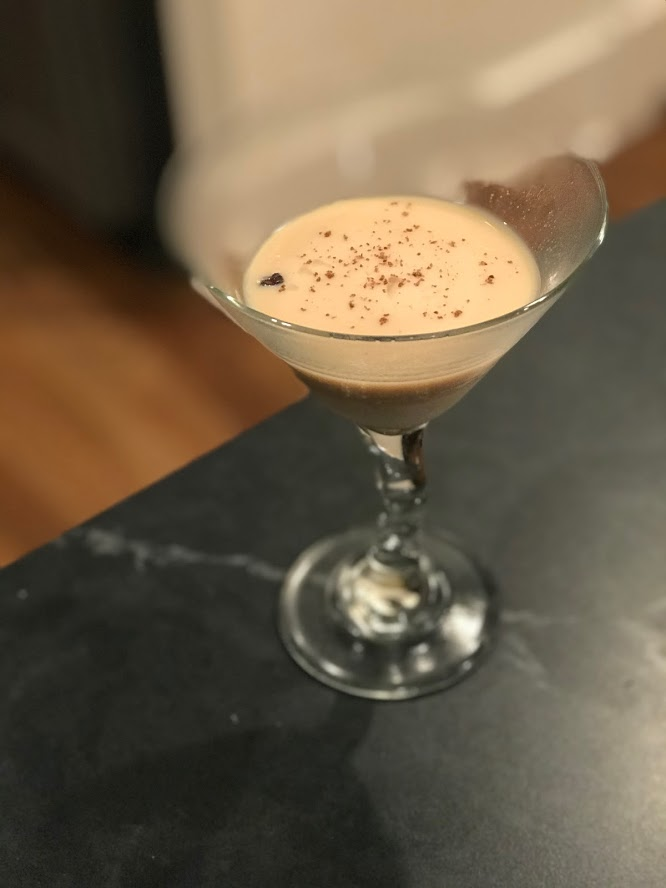
\includegraphics[width=0.65\linewidth]{images/IMG_2914.jpg}
\end{center}
\end{figure}
\newpage
\newrecipe
\begin{recipe}
[
preparationtime = {\unit[1]{h}},
portion = {\portion{3-5}}
]
{Sangria}

\ingredients{
1 (750 ml) bottle red wine\\ 
$\frac{1}{4}$ cup brandy\\ 
$\frac{1}{4}$ cup orange liqueur (Grand Marnier)\\ 
2 tablespoons fresh lime juice\\ 
2 tablespoons fresh orange juice\\ 
$\frac{1}{4}$ cup sugar\\ 
$\frac{1}{2}$ orange, thinly sliced\\ 
$\frac{1}{2}$ lemon, thinly sliced\\ 
1 apple cored and cut into wedges\\ 
1 (750 ml) bottle sparkling water, chilled\\ 
}

\preparation{
\step Combine everything but the sparkling water in a large plastic container or glass pitchers. 
\step Cover the container and chill completely in the fridge, 1 to 2 hours.
\step When ready to serve, add the sparkling water.
}
\end{recipe}

\newrecipe
\begin{recipe}
[
preparationtime = {\unit[2]{h}},
portion = {\portion{6-8}}
]
{White Sangria}

\ingredients{
2 (750 ml) bottles white Spanish wine\\ 
$\frac{1}{2}$ cup Spanish brandy\\ 
$\frac{1}{4}$ cup Spanish orange liqueur\\ 
1 cup pear juice\\ 
$\frac{1}{2}$ cup superfine sugar\\ 
$\frac{1}{2}$ cup sliced pear\\ 
2 apricots\\ 
2 peaches\\ 
$\frac{1}{2}$ pound seedless white grapes\\ 
1 (750 ml) bottle Prosecco, chilled\\ 
}

\preparation{
\step Remove the pits of the apricot and peaches and slice into thin wedges.
\step Combine the wine, brandy, orange liqueur, pear juice, and sugar in a large pitcher and stir until the sugar has dissolved.
\step Add the fruit and stir well to combine.\\ 
\step Cover and refrigerate until well chilled, about 2 hours.
\step Stir in the Prosecco and serve the sangria in large wine glasses, over ice if desired.
}

\hint{
A good Spanish wine could be Albarino (Galacia), Viura (Rioja), or Verdejo (Rueda)
}
\end{recipe}

\newrecipe
\begin{recipe}
[
preparationtime = {\unit[15]{m}},
portion = {\portion{3-4}}
]
{Snowtini}

\ingredients{
1 ounce bittersweet chocolate\\ 
1 $\frac{1}{2}$ cups ice\\ 
3 ounces vanilla vodka\\ 
3 ounces chocolate liqueur (Godiva)\\ 
3 ounces Irish cream (Baileys)\\ 
}

\preparation{
\step Place the martini glasses on a designated, flat shelf in the freezer for 10 minutes.
\step Use a serrated knife, cut shavings off the block of chocolate and reserve for later.
\step Fill a cocktail shaker with ice. Pour the vodka, chocolate liqueur and Irish cream over the ice. Put top on the shaker and shake firmly.
\step Carefully pull out the glasses from the freezer taking care not to get the finger marks on the body of the glass.
\step Pour into chilled glass. Garnish with chocolate shavings in the middle and serve.
}
\end{recipe}



\part{Meats}

\chapter{Beef}
\begin{figure}[h]
\begin{center}
   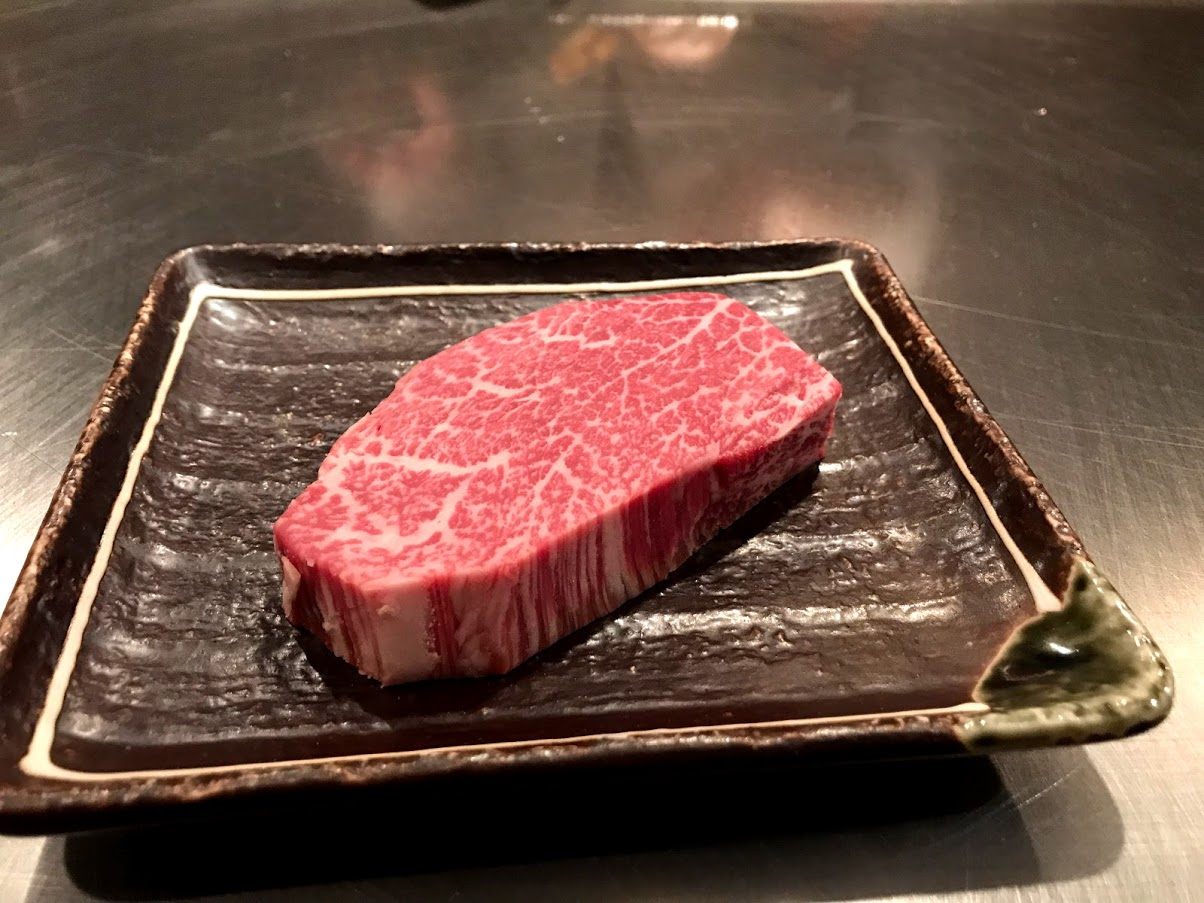
\includegraphics[width=\linewidth]{images/IMG_1345.jpg}
\end{center}
\end{figure}
\newpage
\newrecipe
\begin{recipe}
[
preparationtime = {\unit[30]{m}},
bakingtime = {\unit[1.5]{h}},
portion = {\portion{4-6}},
source = Giada De Laurentiis
]
{Braciole}

\ingredients{
$\frac{1}{2}$ cup dried Italian style bread crumbs\\ 
1 garlic clove, minced\\ 
2/3 cup grated Pecorino Romano\\ 
1/3 cup grated provolone\\ 
2 tablespoons fresh Italian parsley leaves\\ 
4 tablespoons olive oil\\ 
Salt and freshly ground pepper\\ 
1 (1 $\frac{1}{2}$ pound) flank steak\\ 
1 cup dry white wine\\ 
3 $\frac{1}{4}$ cups marinara sauce\\ 
}

\preparation{
\step Chop the parsley leaves finely. Preheat the oven to 350 degrees.
\step Stir the first 5 ingredients (bread crumbs, garlic, Pecorino Romano, provolone, and parsley) in a medium bowl to blend. Stir in 2 tablespoons of the oil.
\step Season the mixture with salt and pepper and set aside.
\step Lay the flank steak flat on the work surface. Sprinkle the bread crumb mixture evenly over the steak to cover the top evenly.
\step Starting at 1 short end, roll up the steak as a jelly roll to enclose the filling completely. 
\step Using butcher's twine, tie the steak roll to secure. Sprinkle the braciole with salt and pepper.
\step Heat the remaining 2 tablespoons of oil in a heavy large ovenproof skillet over medium heat.
\step Add the braciole and cook until browned on all sides, about 8 minutes.\\ 
\step Add the wine to the pan and bring to a boil.\\ 
\step Stir in the marinara sauce. Cover partially with foil and bake until the meat is almost tender, turning the braciole and basting with the sauce every 30 minutes.
\step After 1 hour, uncover and continue baking until the meat is tender, about 30 minutes longer. The total cooking time should be about 1 $\frac{1}{2}$ hours.
\step Remove the braciole from the sauce. Using a large sharp knife, cut the braciole crosswise and diagonally into $\frac{1}{2}$ inch thick slices.
\step Transfer the slices to plates. Spoon the sauce over and serve.
}
\end{recipe}

\newrecipe
\begin{recipe}
[
preparationtime = {\unit[10]{m}},
bakingtime = {\unit[1.5]{h}},
portion = {\portion{6-8}},
source = Harris Teeter
]
{Harris Teeter's Rancher Chuck Roast}

\ingredients{
3 pounds chuck roast\\ 
4 cloves garlic, minced\\ 
1 teaspoon kosher salt\\ 
2 teaspoons parsley\\ 
1 teaspoon ground black pepper\\ 
2 tablespoons shallots, minced\\ 
$\frac{1}{2}$ teaspoon basil, chopped\\ 
$\frac{1}{2}$ teaspoon thyme, chopped\\ 
$\frac{1}{2}$ pound bacon, diced\\ 
$\frac{1}{2}$ teaspoon oregano, chopped\\ 
1 cup red wine\\ 
}

\preparation{
\step Preheat oven to 350 degrees. Place foil in baking dish.
\step Place roast in foil, add salt, pepper, garlic, parsley, and shallots, Italian herbs on top of the roast.
\step Lay the diced bacon strips over the herbs and seasonings.
\step Add 1 cup red wine and wrap foil around the roast tightly.
\step Roast for 1-1 $\frac{1}{2}$ hours.
}
\end{recipe}

\newrecipe
\begin{recipe}
[
preparationtime = {\unit[15]{m}},
bakingtime = {\unit[2]{h}},
portion = {\portion{3-4}},
source = Great Grandma McCollum
]
{Hawaiian Beef}

\ingredients{
2-4 pounds stew meat or cubed chuck steak\\ 
1 $\frac{1}{2}$ tablespoon brown sugar\\ 
$\frac{1}{2}$ teaspoon ginger\\ 
1 teaspoon dry mustard\\ 
1/8 teaspoon pepper\\ 
1 cup tomato sauce\\ 
2 tablespoons lemon juice\\ 
1 cup water\\ 
1 bay leaf\\ 
1 chopped onion\\ 
1 can crushed pineapple\\ 
}

\preparation{
\step Brown Meat.\\ 
\step Combine the rest of the ingredients and heat to make the sauce.
\step Bake the meat and sauce covered 350 degrees 2 hours or in the crockpot on low for several hours.
}
\end{recipe}

\newrecipe
\begin{recipe}
[
preparationtime = {\unit[15]{m}},
bakingtime = {\unit[2]{h}},
portion = {\portion{3-4}},
source = Harris Teeter
]
{Holiday Rib Roast}

\ingredients{
5 rib bone-in rib roast (6 to 8 pounds)\\ 
1 tablespoon Worcestershire sauce\\ 
10 to 12 pounds of rock salt\\ 
1 cup water\\ 
Salt and pepper\\ 
1 large deep disposable aluminum plan\\ 
}

\preparation{
\step Rub rib roast with Worcestershire sauce.\\ 
\step Sprinkle salt and pepper over roast, be sure to cover entire piece of meat.
\step Fill aluminum pan with 2 to 3 inches of rock salt. Place roast in plan bone side down into the rock salt.
\step Pour remaining rock salt completely over roast, be sure to cover the entire piece of meat. Then, pour cup of water over salt. 
\step Place in preheated 500 degree oven for 1 hour.\\ 
\step Turn oven down to 350 degrees and cook 20 minutes to the pound until done.\\ 
\step Remove from oven at the end of cooking cycle and let sit for 5 minutes.\\ 
\step To remove roast from rock salt it might be necessary to break salt with a kitchen hammer.
}
\end{recipe}
\newrecipe
\begin{recipe}
[
preparationtime = {\unit[3]{h}},
bakingtime = {\unit[1.25]{h}},
portion = {\portion{4-6}},
]
{French Dip Sandwiches}

\ingredients{
\textbf{For the onion spread:}\hspace*{\hfill}\\ 
3 tablespoons vegetable oil\\ 
1 large onion, thinly sliced\\ 
kosher salt\\ 
6 medium shallots, thinly sliced\\ 
2 bunches scallions, chopped\\ 
%(white and green parts separated)
1-$\frac{1}{2}$ cups sour cream\\ 
1 cup mayonnaise\\ 
2 teaspoons white wine vinegar\\ 
2 teaspoons Worcestershire sauce\\ 
\\ \textbf{For the sandwiches:}\hspace*{\hfill}\\ 
6 cloves garlic\\ 
kosher salt\\ 
1 teaspoon extra-virgin olive oil\\ 
$\frac{1}{2}$ teaspoon celery salt\\ 
pinch of cayenne pepper\\ 
freshly ground black pepper\\ 
3-4 pound beef eye round roast\\ 
4 cups beef broth\\ 
2 stalks celery, roughly chopped\\ 
3 sprigs parsley\\ 
2 tablespoons butter\\ 
2 tablespoons flour\\ 
2 teaspoons dry sherry\\ 
6 6 inch Italian rolls\\ 
12 slices provolone cheese\\ 
}

\preparation{\\ 
\\ \textbf{Make the onion spread:}
\step Heat the vegetable oil in a large skillet over medium low heat. 
\step Add the onion and pinch of salt; cover and cook, stirring, until golden about 35 minutes.
\step Add the shallots and scallion whites; cover and cook stirring until browned about 25 more minutes.
\step Stir in scallion greens, then remove from the heat and let cool.
\step Chop the onion mixture and transfer to a bowl. Add the sour cream, mayonnaise, vinegar, Worcestershire sauce and 1 teaspoon salt. 
\step Cover and refrigerate at least 2 hours and up to 1 day.
\\ 
\\ \textbf{Make the beef for the sandwiches:}
\step Mince the garlic, then sprinkle with 1 teaspoon salt and mash into a paste with the flat side of a large knife.
\step Transfer to a bowl; add the olive oil, celery salt, cayenne and $\frac{1}{2}$ teaspoon black pepper.
\step Cut small slits all over the beef with a knife, then use your fingers and push the garlic paste into the slits.
\step Cover, refrigerate at least 1 hour or overnight.\\ 
\step Preheat the oven to 425 degrees. Bring the beef to room temperature.
\step Sprinkle with 2 teaspoons salt and $\frac{1}{2}$ teaspoon pepper. 
\step Place on a rack in a roasting pan; add 1 cup broth, $\frac{1}{4}$ cup water, the celery, onion, parsley to the pan.
\step Roast 10 minutes, then reduce the oven temperature to 350 degrees and roast until thermometer inserted into the center of the beef registers 115 degrees about 60 minutes longer.
\step Transfer to a cutting board; let rest 20 minutes. Strain the pan juices; reserve.\\ 
\\ \\ \textbf{Make the jus:}
\step Melt the butter in a medium saucepan over medium heat. Add the flour and cook stirring 1 minute.
\step Whisk in the reserved pan juices and the remaining 3 cups broth and bring to a boil, whisking.
\step Remove the pan from the heat and stir in the sherry.\\ 
\step Split french rolls and put two pieces of provolone cheese on each roll – put in 350 degree oven until the cheese melts.
\step Brush the rolls with some of the onion spread. Thinly slice the beef against the grain.
\step Dunk the slices in the jus, then layer on the rolls. Serve the remaining jus in small bowls for dipping. Remaining onion spread can be used on chips as dip.

}
\end{recipe}


\chapter{Chicken}
\begin{figure}[h]
\begin{center}
   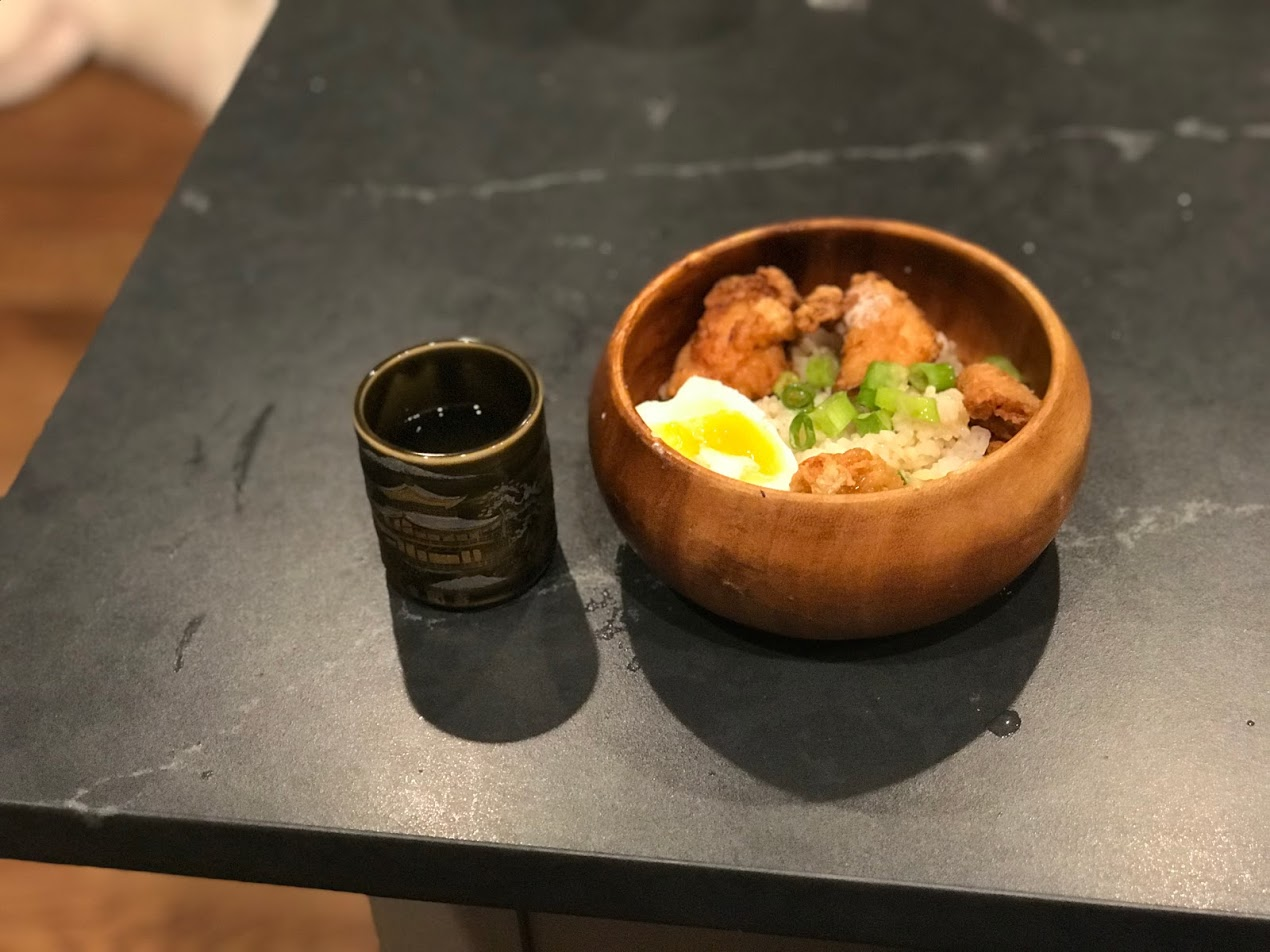
\includegraphics[width=\linewidth]{images/IMG_2109.jpg}
\end{center}
\end{figure}
\newpage
\newrecipe
\begin{recipe}
[
preparationtime = {\unit[2.5]{h}},
portion = {\portion{4-5}},
source = Steve
]
{Karaage (Japanese Fried Chicken)}

\introduction{This is the recipe shown on the Chicken Chapter page. Feel free to add whatever you want to your karaage bowl; bean sprouts, cabbage, and a soft boiled egg are all excellent additions. The recipe for sushi rice can be found on Page~\pageref{pg:sushi_rice}}

\hint{Use a meat thermometer when frying the chicken to make sure to get the perfect temperature. You don't want them to overcook!}

\ingredients{
1 lb skin-on chicken thigh, cubed\\ 
1 tablespoon sake\\ 
1 teaspoon sugar\\ 
2 tablespoons soy sauce\\ 
1 tablespoon ginger, grated\\ 
1 clove garlic, minced\\ 
1 egg, beaten\\ 
$\frac{1}{2}$ cup potato starch\\ 
cooking oil, for frying\\
3 cups sushi rice\\ 
1 green onion\\ 
}

\preparation{
\step In a large bowl, combine the chicken, sake, sugar, soy sauce, ginger, and garlic. Mix well. 
\step Cover the bowl with plastic and marinate for at least 2 hours (up to overnight) in the fridge.
\step Dredge the chicken with the egg and then the potato starch.
\step Heat the oil to 340$^{\circ}$F. Fry the chicken until golden brown and fully cooked, 5-7 minutes. As each one cooks, set it on a drying grate to drip dry.
\step Serve in a bowl with warm rice and green onions.
}
\end{recipe}

\newrecipe
\begin{recipe}
[
preparationtime = {\unit[40]{m}},
bakingtime = {\unit[20]{m}},
portion = {\portion{4-6}},
]
{Chicken Enchiladas}

\ingredients{
2 tablespoons butter\\ 
2 onions, thinly sliced\\ 
2 cups chopped cooked chicken\\ 
$\frac{1}{2}$ cup red pepper\\ 
8 ounces of cream cheese, cubed\\ 
$\frac{1}{4}$ teaspoon salt\\ 
$\frac{1}{4}$ teaspoon pepper\\ 
4 (4.5 ounce) cans diced green chiles\\ 
1 small onion, chopped\\ 
2 garlic cloves, minced\\ 
2 teaspoons dried oregano\\ 
1 teaspoon ground cumin\\ 
$\frac{1}{2}$ teaspoon sugar\\ 
1 (14-1/2 ounce) can chicken broth\\ 
$\frac{1}{2}$ cup green verde salsa\\ 
10 (7 inch) flour tortillas\\ 
2 cups (8 ounces) shredded Mexican cheese\\ 
}

\preparation{
\step Melt butter in a large skillet over medium high heat, stirring often.
\step Add sliced onions and cook 20 minutes or until caramelized.
\step Reduce heat to low and add chopped chicken and next 4 ingredients, stirring until combined. Set aside.
\step Pulse chiles and next 5 ingredients in blender or food processor several times until combined.
\step Bring chile mixture and chicken broth to a boil in a saucepan over high heat; cook 5 minutes or until slightly thickened. (Mixture should be the consistency of a thin gravy.)
\step Remove from heat and stir in salsa.\\ 
\step Spread one third chile mixture evenly on bottom of a lightly greased 13 x 9 inch baking dish.
\step Spoon chicken mixture evenly down center of each tortilla; roll up and place seam side down in prepared baking dish.
\step Top with remaining chile mixture; sprinkle with cheese.\\ 
\step Bake at 375 degrees for 20 to 25 minutes or until bubbly.
}
\end{recipe}

\newrecipe
\begin{recipe}
[
preparationtime = {\unit[2]{h}},
bakingtime = {\unit[55]{m}},
portion = {\portion{6-8}},
]
{Pollo Salsa Verde}

\ingredients{
4 boneless chicken breasts (thin sliced)\\ 
2 medium limes\\ 
1$\frac{1}{3}$ cup verde salsa\\ 
15 8 inch flour tortillas\\ 
$\frac{3}{4}$ cup sour cream\\ 
1 cup grated Monterey jack cheese\\ 
}

\preparation{
\step Place chicken in 9 inch by 12 inch glass baking dish. Squeeze limes over chicken and season to taste with fresh ground pepper and herbs. Marinate for 2 hours.
\step Preheat oven to 350 degrees. Bake chicken uncovered for 20 minutes.
\step Remove from oven and cover chicken evenly with $\frac{2}{3}$ cup salsa.
\step Cut tortillas into 1 inch strips.\\ 
\step Cover the top of the chicken with the strips into a checkerboard pattern, using only half the strips.
\step Spread another 2/3 cup salsa and add another layer of tortillas in the same checkerboard pattern.
\step Cover the tortillas with $\frac{2}{3}$ cup sour cream and bake covered for 20 minutes.\\ 
\step Remove from the oven, add one cup of grated Monterey jack cheese evenly over the top of the tortillas.
\step Return to the oven and broil until the cheese turns golden brown (should be about 15 minutes). 
\step Let stand 10 minutes before serving.
}
\end{recipe}

\newrecipe
\begin{recipe}
[
preparationtime = {\unit[1.25]{h}},
portion = {\portion{4-6}},
source = Giada De Laurentis edited by Mom
]
{Roman style Chicken}

\ingredients{
3 skinless chicken breast halves, with ribs\\ 
4 skinless chicken thighs with bones\\ 
$1\frac{1}{2}$ teaspoon salt\\ 
$1\frac{1}{2}$ teaspoon freshly ground black pepper\\ 
$\frac{1}{4}$ cup olive oil\\ 
1 red bell pepper, sliced\\ 
1 yellow bell pepper, sliced\\ 
3 ounces prosciutto, chopped\\ 
2 cloves garlic, chopped\\ 
1 15 ounce can diced tomatoes\\ 
$\frac{1}{2}$ cup white wine\\ 
1 tablespoon fresh thyme leaves\\ 
1 teaspoon fresh oregano leaves\\ 
$\frac{1}{2}$ cup chicken broth\\ 
$\frac{1}{4}$ cup chopped fresh parsley leaves\\ 
Fresh Parmesan cheese\\ 
1 box fettuccine\\ 
}

\preparation{
\step Season the chicken with $\frac{1}{2}$ teaspoon salt and $\frac{1}{2}$ teaspoon pepper. \step In a heavy large skillet, heat the olive oil over medium heat.
\step When the oil is hot, cook the chicken until browned on both sides.
\step Remove chicken from the pan and set aside -- cover with foil or large boil to keep hot.
\step Keeping the same pan over medium heat, add the peppers and prosciutto and cook until the peppers have browned and the prosciutto is crisp, about 5 minutes.
\step Add the garlic and cook for 1 minute.\\ 
\step Add the tomatoes, wine and herbs. Then, using a wooden spoon, scrape the browned bits off the bottom of the pan. 
\step Return the chicken to the pan, add the stock and bring the mixture to a boil.
\step Reduce the heat and simmer covered, until the chicken is cooked through, about 20 to 30 minutes.
\step Meanwhile, cook the fettuccine and drain.\\ 
\step Add the fettuccine to a large pasta bowl. Add chicken over the top.\\ 
\step Sprinkle with fresh Parmesan cheese and chopped parsley leaves.
}
\end{recipe}

\newrecipe
\begin{recipe}
[
preparationtime = {\unit[50]{m}},
portion = {\portion{4-6}},
source = Mom
]
{Chicken Marsala}

\ingredients{
\item 1 pound thin chicken\\ 
\item $\frac{3}{4}$ cup Italian bread crumbs\\ 
\item $\frac{1}{2}$ cup milk\\ 
\item 1 egg\\ 
\item 8 ounces mushrooms\\ 
\item 1 small onion, diced\\ 
\item 2 tablespoons olive oil\\ 
\item 2 tablespoons butter\\ 
\item 1 cup Marsala\\ 
\item $\frac{1}{2}$ tablespoon of rosemary\\ 
}

\preparation{
\step If chicken isn't thinned already, beat thin with a meat mallet.
\step Heat olive oil in skillet over medium heat.\\ 
\step In a small bowl, beat egg and add milk. In another small bowl or small plate, add bread crumbs.
\step Dredge chicken in milk and egg mixture and coat with bread crumbs and put in skillet.
\step When brown (about 3 to 4 minutes), turn over another 3 to 4 minutes).
\step Remove chicken from pan and plate it.\\ 
\step Turn up heat to medium high and in skillet melt butter, add mushrooms and onion and cook until soft several minutes.
\step Add Marsala wine and rosemary.\\ 
\step Return chicken to pan, turn down heat back to medium, and cook a couple of minutes on each side.
}
\end{recipe}

\newrecipe
\begin{recipe}
[
preparationtime = {\unit[8.5]{h}},
portion = {\portion{4-5}},
]
{Slow cooker Chicken Paprikash}

\ingredients{
3 tablespoons all purpose flour\\ 
2 pounds boneless, skinless chicken breasts\\ 
1 $\frac{1}{4}$ cups chicken stock\\ 
8 ounces mushrooms, sliced\\ 
1 large onion, chopped\\ 
1 cup chopped red bell pepper\\ 
$\frac{1}{2}$ cup shredded carrot\\ 
2 large garlic cloves, minced\\ 
2 tablespoons Hungarian sweet paprika\\ 
1 teaspoon salt\\ 
1 teaspoon freshly ground black pepper\\ 
1 $\frac{1}{4}$ cups sour cream\\ 
}

\preparation{
\step Rinse chicken breasts and pat dry, then cut into $\frac{1}{2}$ inch strips.
\step In a bowl, combine the flour and chicken, tossing well to coat.
\step In a slow cooker, combine the chicken mixture, stock, mushrooms, onion, bell pepper, carrot, garlic, paprika, salt and pepper.
\step Cover and cook on low heat for 8 hours.\\ 
\step Just before serving, stir in the sour cream.\\ 
\step Serve with egg noodles, mashed potatoes, or orzo.
}
\end{recipe}


\chapter{Pork}
\begin{figure}[h]
\begin{center}
   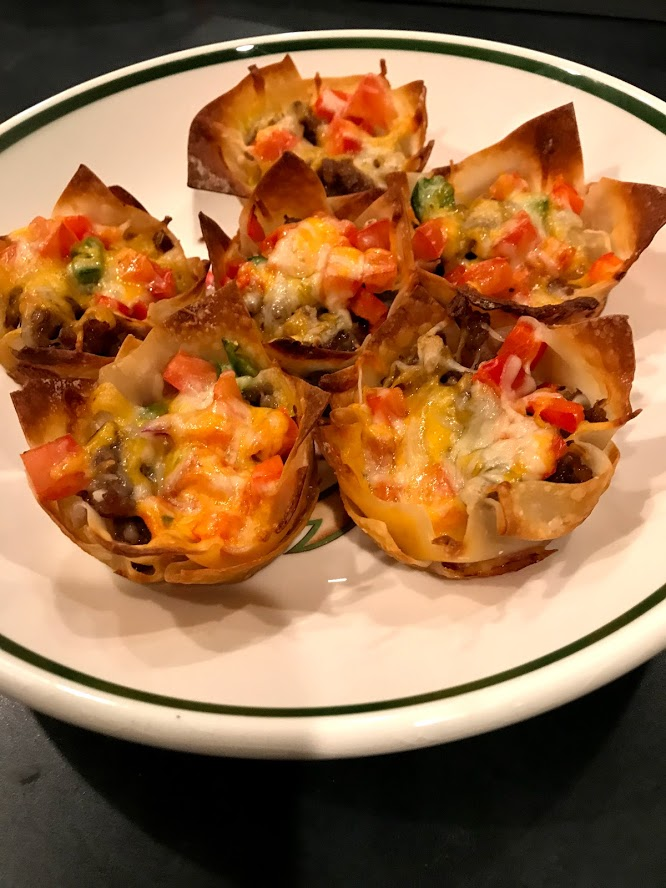
\includegraphics[width=0.65\linewidth]{images/IMG_2918.jpg}
\end{center}
\end{figure}
\newpage
\newrecipe
\begin{recipe}
[
preparationtime = {\unit[20]{m}},
bakingtime = {\unit[15]{m}},
portion = {\portion{4-8}},
source = Steve
]
{Wonton Poppers}

\hint{This is the recipe shown on the Chicken Chapter page. Feel free to add whatever you want to the wontons to make your own spin on them. Cream cheese can also be used in these to cut the heat some.}

\ingredients{
1 package wonton wrappers\\ 
1 Fresh jalapeno\\ 
1 lb ground pork\\ 
8 ounces Mexican or Colby jack cheese\\ 
2 tomatoes\\ 
1 green bell pepper\\ 
handful of cilantro\\ 
2 avocados\\ 
$\frac{1}{2}$ tablespoon crushed red pepper\\ 
1 teaspoon salt\\ 
1 teaspoon pepper\\ 
}

\preparation{
\step Dice the tomato, cilantro, bell pepper, and jalapeno and mix together.
\step Sprinkle the sausage with red pepper, salt, and pepper. Then brown it over medium-high heat.
\step Put each wonton into the holes in a cupcake or muffin tin (spray with oil if it isn't non-stick).
\step Put sausage and a sprinkle of cheese in each wonton before covering that with another wonton.
\step Sprinkle mixed vegetables from step 1 on top of top wonton before covering with even more cheese.
\step Bake for 10-15 minutes until wonton edges are golden brown. Then, serve with sliced avocado. 

}
\end{recipe}

\newrecipe
\begin{recipe}
[
preparationtime = {\unit[1.1]{h}},
bakingtime = {\unit[30]{m}},
portion = {\portion{5-6}},
]
{Asian Pork Tenderloin}

\ingredients{
$\frac{1}{2}$ cup soy sauce\\ 
$\frac{1}{4}$ cup pineapple juice\\ 
$\frac{1}{4}$ cup coarsely chopped green onions\\ 
$\frac{1}{4}$ cup coarsely chopped shallots\\ 
2 tablespoons coarsely chopped fresh ginger\\ 
2 tablespoons honey\\ 
2 tablespoons rice wine vinegar\\ 
1 tablespoon essence\\ 
$\frac{1}{2}$ teaspoon cinnamon\\ 
$\frac{1}{2}$ teaspoon nutmeg\\ 
2 tablespoons chopped garlic\\ 
1 tablespoon sesame oil\\ 
1 tablespoon crushed red pepper\\ 
2 pork tenderloins (about 2 pounds)\\ 
}

\preparation{
\step Combine all the ingredients except the tenderloins in a food processor and pulse several times to puree in order to make the marinade.
\step Put the tenderloins in a large plastic bag and pour in the marinade.
\step Seal the bag and refrigerate for 1 hour.\\ 
\step Preheat the oven to 400 degrees.\\ 
\step Heat a large nonstick skillet over high heat.\\ 
\step When the skillet is hot, add the tenderloins and sear, turning to ensure even browning, about 4 minutes.
\step Transfer to a oven safe dish oiled with olive oil and put in oven.
\step Cook for 30 minutes or until an instant-read thermometer reads 145 degrees.
\step Remove from the oven and let rest for 5 minutes, then serve.
}
\end{recipe}

\newrecipe
\begin{recipe}
[
preparationtime = {\unit[1]{h}},
portion = {\portion{20}},
source = Emeril Lagasse
]
{Pork Egg Rolls with Sweet and Sour Sauce}

\ingredients{
2 tablespoons vegetable oil\\ 
1 pound ground pork\\ 
$\frac{1}{2}$ cup minced onion\\ 
1 tablespoon chopped garlic\\ 
1 pound bok choy, shredded\\ 
$\frac{1}{2}$ pound medium shrimp\\ 
1 tablespoon dark sesame oil\\ 
Soy sauce to taste\\ 
$\frac{1}{4}$ cup sake (optional)\\ 
1 tablespoon sugar\\ 
1 pound fresh bean sprouts\\ 
$\frac{1}{4}$ cup green onions, green part only\\ 
20 (6 inch) egg roll wrappers\\ 
1 egg beaten for egg wash\\ 
Oil for frying\\ 
}

\preparation{
\step  Preheat the fryer. If not done already, peel, devein and chop shrimp and wash and pat down bean sprouts.
\step In a wok, heat the oil. When the oil is hot, add the pork. Season with salt and pepper. Stir fry for 3 minutes.
\step Add the onions and garlic, continue to cook for 2 minutes.
\step Add the bok choy and shrimp. and season with salt and pepper. Stir-fry for 1 minute. Season with the sesame oil, soy sauce, sake and sugar.
\step Add the sprouts and green onions and mix thoroughly. Remove from the heat and cool completely.
\step To assemble, spoon about $\frac{1}{4}$ cup of the filling in a rectangular shape on the center of each wrapper. Then, fold in the ends toward the center about $\frac{1}{4}$ inch. 
\step Beginning at the bottom roll up the wrapper, like a jelly roll, using a little of the egg wash to seal the end tightly.
\step Repeat until all of the egg rolls are done.\\ 
\step Fry the egg rolls in batches until golden brown stirring occasionally for overall browning, about 2 to 3 minutes.s
\step Remove from the oil and drain on paper towels. Season with essence.\\ 
\step Serve warm with sweet and sour sauce.
}
\end{recipe}

\newrecipe
\begin{recipe}
[
preparationtime = {\unit[1.25]{h}},
bakingtime = {\unit[45]{m}},
portion = {\portion{8-12}},
source = Emeril Lagasse
]
{Double Cut Pork Chops with Caramelized Onion Gravy and Pecan Glazed Sweet Potatoes}

\ingredients{
\textbf{Caramelized onion gravy:}\hspace*{\hfill}\\ 
2 tablespoons butter\\ 
3 cups thinly sliced onions\\ 
1 tablespoon light brown sugar\\ 
1 teaspoon garlic\\ 
1 teaspoon thyme leaves\\ 
2 tablespoons all-purpose flour\\ 
1 cup chicken stock\\ 
Salt \& pepper\\ 
\\ 
\textbf{Pecan Glazed Sweet Potatoes:}\hspace*{\hfill}\\ 
1 $\frac{1}{2}$ pounds sweet potatoes\\ 
1 tablespoon olive oil\\ 
Salt and pepper\\ 
6 tablespoons butter\\ 
$\frac{1}{2}$ cup light brown sugar\\ 
$\frac{1}{2}$ cup pecans\\ 
\\ 
\textbf{Pork chops:}\hspace*{\hfill}\\ 
4 double cut bone in pork chops\\ 
1 tablespoon essence\\ 
2 teaspoons salt\\ 
2 tablespoons olive oil.\\ 
}

\preparation{
\\ \textbf{Gravy:}
\step In a small saucepan set over medium heat, add the butter.
\step Once melted, add the onions and sugar to the pan and sweat, stirring occasionally until wilted and well caramelized, about 18 to 20 minutes.
\step Add the garlic and thyme to the pan and saut\'{e} until fragrant, about 30 seconds.
\step Add the flour to the pan and stir to make a roux, about 2 to 3 minutes.
\step Add the chicken stock. Bring to a boil and reduce heat to a simmer for 15 minutes and season with the salt and pepper.\\ 
\\ \textbf{Sweet potatoes:}
\step Wash the sweet potatoes and peel. Chop the sweet potatoes into 1 inch pieces and place in a roasting pan. Drizzle with the olive oil and season with the salt and pepper.
\step Place the potatoes in the oven and roast until tender about 30 minutes. Remove from the oven and set aside.
\step In a large 12 inch saut\'{e} pan, add the butter and brown sugar.
\step When the butter begins to boil with the sugar, add the pecans and the sweet potatoes. 
\step Continue to cook, tossing occasionally, until the potatoes are well glazed, about 3 minutes.\\ 
\\ \textbf{Pork chops:}
\step Preheat the oven to 400 degrees. Set a large 12inch saut\'{e} pan over medium-high heat.
\step Add the olive oil to the pan and once hot, place the pork chops in the pan. Sear the pork chops until well caramelized about 5 minutes.
\step Turn over and sear on the second side for an additional 5 minutes.\\ 
\step Remove the pan from the stove top and place in the oven. Roast the pork chops until a thermometer reaches 150 degrees about 10 to 12 minutes for medium.
\step Remove the chops from the oven and serve with the glazed sweet potatoes and the caramelized onion gravy.
\step Garnish with chopped parsley.
}
\end{recipe}

\begin{recipe}
[
preparationtime = {\unit[1]{h}},
portion = {\portion{4-6}},
]
{Pork Chops, Cabbage and Apples}

% or 1 teaspoon dried thyme
%  or 1 teaspoon dried sage
\ingredients{
3 teaspoons paprika\\
2 teaspoons fresh chopped thyme\\ 
2 teaspoons kosher salt\\ 
1 $\frac{1}{2}$ teaspoon fresh chopped sage\\ 
6 (1/2 inch thick) pork loin chops\\ 
2 bacon slices\\ 
1 head cabbage coarsely chopped\\ 
2 medium onions, thinly sliced\\ 
1 large Granny Smith apple\\ 
1 tablespoon tomato paste\\ 
1 (12 ounce) bottle lager beer\\ 
}

\preparation{
\step Wash, peel, and slice the apple.\\
\step Combine 2 teaspoons paprika, 1 teaspoon fresh or $\frac{1}{2}$ teaspoon dried thyme, 1 teaspoon salt, 1 teaspoon pepper and 1 teaspoon fresh or $\frac{1}{2}$ teaspoon dried sage, rub evenly overly pork chops.
\step Cook bacon slices in large, deep skillet over medium high heat 6 to 8 minutes or until crisp; remove bacon and drain on paper towels, reserving drippings in skillet.
\step Crumble bacon up when cool enough.\\ 
\step Cook pork in hot drippings 3 minutes on each side or until browned and done; remove pork from pan and keep warm.
\step Add cabbage, onions and apple to pan. Cover and reduce heat to medium; cook stirring occasionally 15 minutes or until cabbage begins to wilt.
\step Add tomato paste, beer, the crumbled bacon, 1 teaspoon paprika, 1 teaspoon fresh or $\frac{1}{2}$ teaspoon dried thyme, 1 teaspoon salt, $\frac{1}{2}$ teaspoon pepper and 1 teaspoon fresh or $\frac{1}{2}$ teaspoon dried sage, stirring to loosen particles from bottom of skillet.
\step Cover and cook 15 minutes or until cabbage is tender and liquid is slightly thickened.\\ 
\step Add pork, and cook uncovered 5 minutes or until thoroughly heated.
}

\hint{
Instead of the fresh thyme, you can use 1 teaspoon dried thyme and instead of fresh sage, you can use 1 teaspoon dried sage.}

\end{recipe}

\newrecipe
\begin{recipe}
[
preparationtime = {\unit[10]{m}},
bakingtime = {\unit[8]{h}},
portion = {\portion{4-6}},
]
{Pulled Pork BBQ}

\ingredients{
1 can Root Beer\\ 
BBQ Rub\\ 
1/3 bottle of BBQ sauce\\ 
2 lbs pork roast (end piece)\\ 
}

\preparation{
\step Empty root beer at bottom on crock pot. Sprinkle BBQ rub on pork roast and put it crockpot.
\step Pour BBQ sauce on top of roast. Cook low for 8 hours or more.
}
\end{recipe}

\newrecipe
\begin{recipe}
[
preparationtime = {\unit[45]{m}},
bakingtime = {\unit[1.5]{h}},
portion = {\portion{10-12}},
]
{Sugarcane Baked Ham with Spiced Apples and Pears}

\hint{The ham should be about 8-10 pounds and spiral sliced}

\ingredients{
12 sugarcane swizzle sticks\\
%, each cut into about 3 inch pieces
1 hickory smoked ham (no bone, cooked)\\ 
% 8-10 pounds spiral slice ham
1 $\frac{1}{2}$ pound ($\sim$4) Granny Smith apples\\ 
1 $\frac{1}{2}$ pound ($\sim$4) Bartlett pears\\ 
\\ \textbf{Glaze:}\hspace*{\hfill}\\ 
1 cup firmly packed light brown sugar\\ 
1 cup Steens 100\% Pure Cane Syrup\\ 
$\frac{1}{2}$ cup dark molasses\\ 
$\frac{1}{2}$ cup dark corn syrup\\ 
1/8 teaspoon freshly grated nutmeg\\ 
$\frac{1}{4}$ teaspoon ground cloves\\ 
1/8 teaspoon ground allspice\\ 
$\frac{1}{2}$ teaspoon ground cinnamon\\ 
1 teaspoon dried mustard\\ 
$\frac{1}{4}$ cup water\\ 
}

\preparation{
\step Preheat oven to 350 degrees. Line a shallow baking pan with parchment or waxed paper.
\step Cut the sugarcane sticks each into about 3 pieces then insert the sugarcane sticks into the ham at 3 to 4 inch intervals. 
\step Tie the ham, using kitchen twine, horizontally and vertically, like a package to hold it together. Place it on a wire rack in the baking pan.
\step In a mixing bowl, combine all the glaze ingredients together except for the mustard and water; mix well. 
\step In a small bowl, dissolve the mustard in the water, then add to the spice mixture; blend well.
\step Brush the entire ham with the glaze, coating it evenly.
\step Wash, core and halve the fruit. Place all around the ham.
\step Baste the ham a second time and baste the fruit with the glaze.
\step  Bake for 45 minutes. Then baste the ham and fruit again. Bake another 45 minutes. Then remove the ham from the oven and let is rest for 5 minutes.
\step Remove and discard the string and swizzle sticks. Then serve the apples and pears on a platter with the ham.
}
\end{recipe}

\newrecipe
\begin{recipe}
[
preparationtime = {\unit[35]{m}},
bakingtime = {\unit[1-3]{h}},
portion = {\portion{4-5}},
source = Aunt Zina
]
{Sweet and Sour Sausage}

\ingredients{
2 pounds polish sausage\\ 
2 cups brown sugar\\ 
$\frac{1}{4}$ cup vinegar\\ 
$\frac{1}{4}$ cup sweet pickle juice\\ 
}

\preparation{
\step Cut sausage in chunks. Boil $\frac{1}{2}$ hour.\\ 
\step Place boiled sausage in shallow baking dish. Add other ingredients.
\step Bake at 350 degrees for 1 hour or put all ingredients in crockpot and cook for approximately 3 hours on low.
}
\end{recipe}

\newrecipe
\begin{recipe}
[
preparationtime = {\unit[2]{h}},
bakingtime = {\unit[30]{m}},
portion = {\portion{4}},
sorurce = Smitten Kitchen
]
{Pancetta, White bean, and Chard Pot Pie}

\ingredients{
\textbf{For the lid:}\hspace*{\hfill}\\ 
2 cups all-purpose flour\\ 
1/2 teaspoon table salt\\ 
13 tablespoons cold unsalted butter\\ 
%, diced
6 tablespoons (90 grams) sour cream\\ 
%or whole Greek yogurt\\ 
1 tablespoon (15 ml) white wine vinegar\\ 
1/4 cup (60 ml) ice water\\ 
1 egg\\ 
1 tablespoon water\\ 
% Beat top two together for egg wash
\textbf{For the filling:}\hspace*{\hfill}\\ 
2 tablespoons (30 ml) olive oil\\ 
4 ounces 1/4-inch-diced pancetta\\ 
1 large or 2 small onions, finely chopped\\ 
1 large carrot, finely chopped\\ 
1 large stalk celery, finely chopped\\ 
Pinch of red pepper flakes\\ 
Salt and freshly ground black pepper\\ 
2 garlic cloves, minced\\ 
8-10 ounce Swiss chard \\ 
%Thinly sliced Swiss chard leaves from an (225- to 285-gram)
%bundle (4 cups); if leaves are very wide, you can halve them lengthwise
3 1/2 tablespoons butter\\ 
3 1/2 tablespoons all-purpose flour\\ 
3 1/2 cups chicken broth\\ 
2 cups cooked and drained white beans\\ 
%cooked and drained, or from one and a third 15.5- ounce (440-gram) cans
}

\hint{You can prepare most of this in advance and place in the fridge to ease cooking time.}

\preparation{
\\ \\ \textbf{Make lids:}
\step In a large, wide bowl, combine the flour and salt. Add the butter and, using a pastry blender, cut them up and into the flour mixture until it resembles little pebbles. 
\step Keep breaking up the bits of butter until the texture is like uncooked couscous.
\step In a small dish, whisk together the sour cream, vinegar, and water, and combine it with the butter-flour mixture.
\step Using a flexible spatula, stir the wet and the dry together until a craggy dough forms. If needed, get your hands into the bowl to knead it a few times into one big ball. 
\step Pat it into a flattish ball, wrap it in plastic wrap, and chill it in the fridge for 1 hour or up to 2 days (it will last a couple months in the freezer).

\\ \textbf{Make filling:}
\step Heat 1 tablespoon olive oil over medium-high heat in a large, wide saucepan, and then add the pancetta.
\step Brown the pancetta, turning it frequently, so that it colors and crisps on all sides; this takes about 10 minutes. Remove it with a slotted spoon, and drain it on paper towels before transferring to a medium bowl.
\step Leave the heat on and the renderings in the pan. Then add an additional tablespoon of olive oil if needed and heat it until it is shimmering.
\step Add onions, carrot, celery, red pepper flakes, and a few pinches of salt, and cook over medium heat until the vegetables are softened and begin to take on color, about 7 to 8 minutes.
\step Add the garlic, and cook for 1 minute more.\\ 
\step Thinly slice the chard, add, and cook until wilted, about 2 to 3 minutes. Season with the additional salt and freshly ground black pepper to taste.
\step Transfer all of the cooked vegetables to the bowl with the pancetta, and set aside.\\ 

\\ \textbf{Make sauce:}
\step Wipe out the large saucepan; don’t worry if any bits remain stuck to the bottom. Then melt the butter in the saucepan over medium-low heat.
\step Add the flour, and stir with a whisk until combined. Continue cooking for 2 minutes, stirring the whole time, until it begins to take on a little color.
\step Whisk in the broth, one ladleful at a time, mixing completely between additions. Once you’ve added one- third of the broth, you can begin to add the rest more quickly, two to three ladlefuls at a time.

\step Once all of the broth is added, stirring the whole time, bring the mixture to a boil and reduce it to a simmer.
\step Cook the sauce until it is thickened and gravylike, about 10 minutes. Season with salt and pepper.
\step Stir the white beans and reserved vegetables into the sauce.\\ 

\\ \textbf{Assemble and cook pot pies:}\\ 
\step Preheat your oven to 375 degrees. Divide the filling between four ovenproof 2-cup bowls. (You’ll have about 1 1/2 cups filling in each.)
\step Set the bowls on a baking pan. Divide the dough into four pieces, and roll it out into rounds that will cover your bowls with an overhang, or about 1 inch wider in diameter than your bowls. 
\step Whisk the egg and tablespoon of water to make an egg wash and brush it lightly around the top rim of your bowls and drape the pastry over each, pressing gently to adhere it. 
\step Brush the lids with egg wash, then cut small, decorative vents in each to help steam escape. 
\step Bake until crust is lightly bronzed and filling is bubbling, about 30 to 35 minutes.
}
\end{recipe}


% Below is how to automate input. But lets do it manually in case we want to rearrange.
%\foreach \i in {01, 02, 03, 04, 05, 06, 07, 08, 09, 10, ...,99} {%
%    \edef\FileName{Recipes/Desserts/\i}%     The % here are necessary to eliminate any
%    \IfFileExists{\FileName}{%  spurious spaces that may get inserted
%       \input{\FileName}%       at these points
%    }
%}

\chapter{Seafood}
\begin{figure}[h]
\begin{center}
   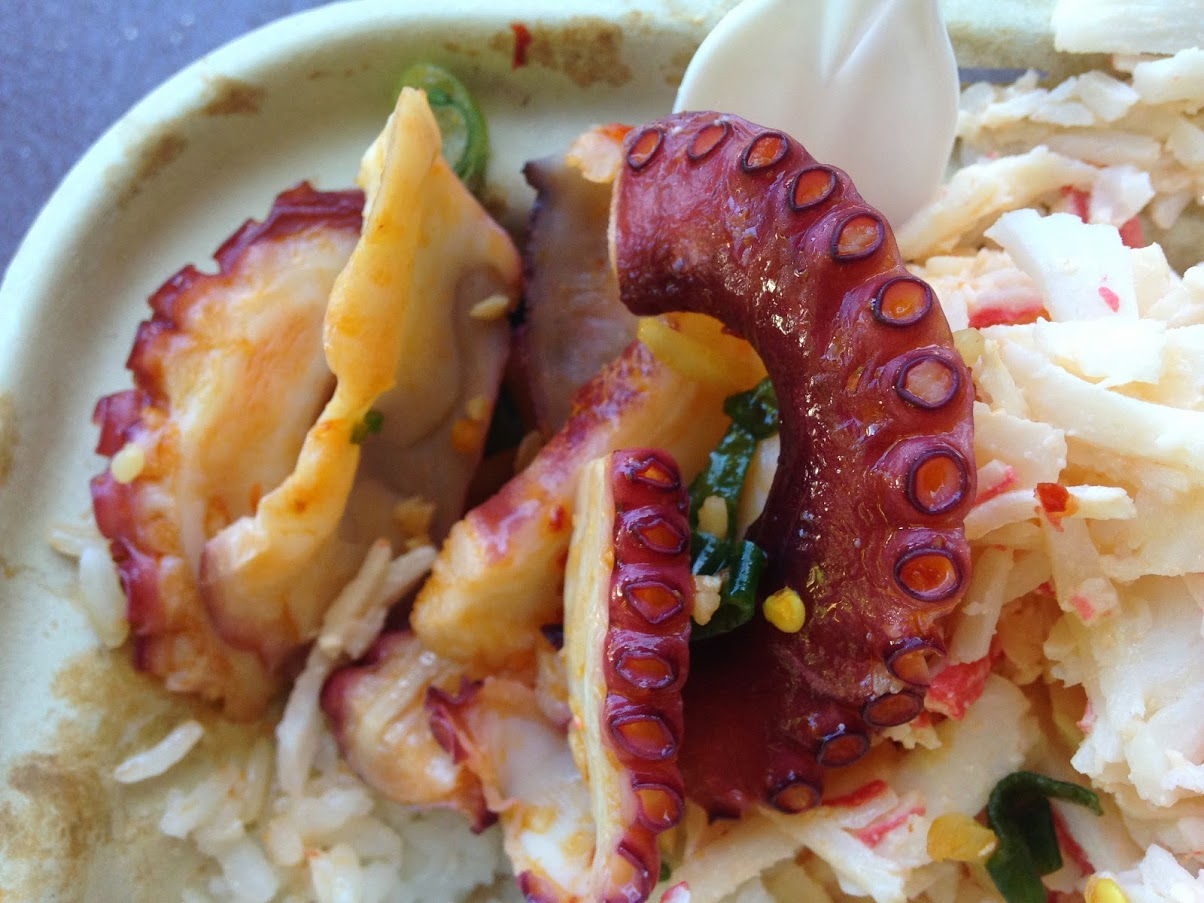
\includegraphics[width=\linewidth]{images/IMG_0456.JPG}
\end{center}
\end{figure}
\newpage
\newrecipe
\begin{recipe}
[
preparationtime = {\unit[20]{m}},
portion = {\portion{2}},
source = Steve
]
{Poke Bowls}

\introduction{Poke is a traditional Hawaiian dish made with raw tuna (sometimes other fish as well) and toppings. This can be a hard dish to make outside of the coast has good quality raw fish is hard to come by. Japanese grocery stores like Tomato are a good place to look for this. Alternatively, you can still used cooked fish. The picture in the Seafood Chapter introduction is a poke bowl with cooked octopus! The recipe for sushi rice can be found on Page~\pageref{pg:sushi_rice}}

\hint{Sriracha mayo is also excellent in the Karaage bowl recipe and other rice dishes. It can be made by mixing 1 teaspoon sriracha with every tablespoon of mayonnaise. See the sushi rice recipe for more details on the rice.}

\ingredients{
1/2 pound sushi grade tuna\\ 
1/4 cup sliced scallions\\ 
2 tablespoons soy sauce\\ 
1 teaspoon sesame oil\\ 
2 tablespoons sriracha mayo\\ 
1 cup sushi rice\\ 
$\frac{1}{2}$ medium avocado\\ 
2 sliced scallions\\ 
}

\preparation{
\step Cut the fish into 1/2-inch cubes while preparing your sushi rice.
\step In a medium bowl, toss tuna with scallions, soy sauce, and sesame oil and sriracha.
\step Put rice in two bowls and then layer the tuna and avocado. Drizzle with spicy mayo to serve.
}
\end{recipe}

\newrecipe
\begin{recipe}
[
preparationtime = {\unit[25]{m}},
portion = {\portion{3-4}},
]
{Sushi Rice}\label{pg:sushi_rice}

\ingredients{
2 cups glutinous white rice (sushi rice)\\ 
3 cups water\\ 
$\frac{1}{2}$ cup rice vinegar\\ 
1 tablespoon vegetable oil\\ 
$\frac{1}{4}$ cup sugar\\ 
1 teaspoon salt\\ 
}

\hint{You can also use a pressure cooker to easily prepare this and avoid the saucepan.}

\preparation{
\step Rinse the rice in a strainer or colander until the water runs clear. 
\step Combine with water in a medium saucepan. Bring to a boil, then reduce the heat to low, cover and cook for 20 minutes. Rice should be tender and water should be absorbed.
\step In a small saucepan, combine the rice vinegar, oil, sugar and salt. Cook over medium heat until the sugar dissolves. 
\step Cool the mixture, then stir into the warm cooked rice. When you pour this in to the rice it will seem very wet. Keep stirring and the rice will dry as it cools.
}
\end{recipe}

\newrecipe
\begin{recipe}
[
preparationtime = {\unit[20]{m}},
portion = {\portion{4}},
]
{Batter Fried Grouper Sandwiches}

\ingredients{
1 cup all purpose flour\\ 
$\frac{1}{4}$ cup cornstarch\\ 
1 tablespoon garlic powder\\ 
$\frac{1}{2}$ teaspoon pepper\\ 
4 (4 ounce) grouper fillets\\ 
$\frac{1}{2}$ to $\frac{3}{4}$ cup buttermilk\\ 
4 onion sandwich buns, toasted\\ 
Oil for frying\\ 
}

\preparation{
\step Combine first 4 ingredients in a shallow dish to make flour mixture (1 cup flour, $\frac{1}{4}$ cup cornstarch, 1 tablespoon garlic powder, $\frac{1}{2}$ teaspoon pepper).
\step Dredge grouper in flour mixture, dip in buttermilk and dredge in flour mixture again.
\step Heat fryer to 350 degrees. Fry fillets in hot oil 5 minutes or until golden; drain on paper towels.
\step Place each fillet on a bun and add desired toppings.
}
\end{recipe}

\newrecipe
\begin{recipe}
[
preparationtime = {\unit[20]{m}},
portion = {\portion{4}},
]
{Jambalaya}

\hint{Buy the shrimp peeled, deveined, and chopped if you don't want to do it yourself.}

\ingredients{
12 medium shrimp\\ 
4 ounces chicken, diced\\ 
1 tablespoon Creole seasoning\\ 
2 tablespoons olive oil\\ 
$\frac{1}{4}$ cup chopped onion\\ 
$\frac{1}{4}$ cup chopped green bell pepper\\ 
$\frac{1}{4}$ cup chopped celery\\ 
2 tablespoons chopped garlic\\ 
$\frac{1}{2}$ cup chopped tomatoes\\ 
3 bay leaves\\ 
1 teaspoon worcestershire sauce\\ 
1 teaspoon hot sauce\\ 
$\frac{3}{4}$ cup rice\\ 
3 cups chicken stock\\ 
5 ounces Andouille sausage, sliced\\ 
Salt and pepper\\ 
}

\preparation{
\step If not already done, peel, devein, and chop the shrimp.
\step In a bowl combine the chopped shrimp, chicken and 1 tablespoon Creole seasoning and work in seasoning well. Set aside.
\step In a large saucepan heat oil over high heat with onion, pepper and celery; cook about 3 minutes.
\step Add garlic, tomatoes, bay leaves, Worcestershire and hot sauces. Stir in rice and slowly add broth.
\step Reduce heat to medium and cook until rice absorbs liquid and becomes tender, stirring occasionally, about 15 minutes.
\step When rice is just tender, add shrimp and chicken mixture as well as the sausage. Cook until meat is done, about 10 minutes more.
\step Season to taste with salt, pepper, and extra Creole seasoning.
}
\end{recipe}

\newrecipe
\begin{recipe}
[
preparationtime = {\unit[40]{m}},
portion = {\portion{4-6}},
]
{Shrimp Boil}

\ingredients{
1 bottle of beer (any kind)\\ 
2 teaspoons kosher salt\\ 
2 lemons, halved\\ 
3 bay leaves\\ 
1 handful of fresh thyme sprigs\\ 
1 head of garlic split horizontally\\ 
1 tablespoon old bay seasoning\\ 
2 pounds jumbo shrimp with shells\\ 
}

\preparation{
\step Fill a large pot with about 2 quarts of water and bottle of beer.
\step Add salt and squeeze in lemon juice from the lemons. Then add the lemons halves, herbs, garlic and old bay.
\step Bring to a boil of medium high heat and simmer for 5 minutes to infuse the water with the aromatics.
\step Reduce the heat to medium low and put shrimp in. simmer, uncovered for 2 to 3 minutes or until shrimp are bright pink.
\step Drain then transfer to a bowl. Chill thoroughly and then peel.
}
\end{recipe}

\newrecipe
\begin{recipe}
[
preparationtime = {\unit[40]{m}},
portion = {\portion{4-6}},
]
{Shrimp Po'Bubba's}

\hint{Buy the shrimp peeled and deveined if you don't want to do it yourself.}

\ingredients{
2 pounds uncooked shrimp\\ 
Salt and freshly ground black pepper\\ 
3 eggs\\ 
$\frac{1}{4}$ cup water\\ 
$\frac{1}{2}$ cup hot sauce\\ 
Oil for frying\\ 
2 cups fry mix (below)\\ 
\\ \textbf{Uncle Bubba's Fry Mix:}\hspace*{\hfill}\\ 
6 cups self-rising flour\\ 
1 cup cornmeal\\ 
1 teaspoon salt\\ 
1 teaspoon pepper\\ 
}

\preparation{
\step For fry mix, mix ingredients together and store in an airtight container for up to 4 months.
\step If not already done, peel, devein, and butterfly the shrimp. Then lightly sprinkle with salt and pepper. 
\step Heat Fryer to 350 degrees.\\ 
\step In a small bowl mix the eggs, $\frac{1}{4}$ cup water and hot sauce.
\step Place the fry mix in a shallow dish. Dip each shrimp in the egg mixture and then into the fry mix.
\step Place the shrimp in the fryer and fry until golden brown, about 2 minutes. Remove with a strainer and drain on paper towels for a minute.
\step Serve on toasted hoagie roll with whatever toppings are desired.
}
\end{recipe}


\part{Pasta and Pizzas}

\chapter{Pasta}
\begin{figure}[h]
\begin{center}
   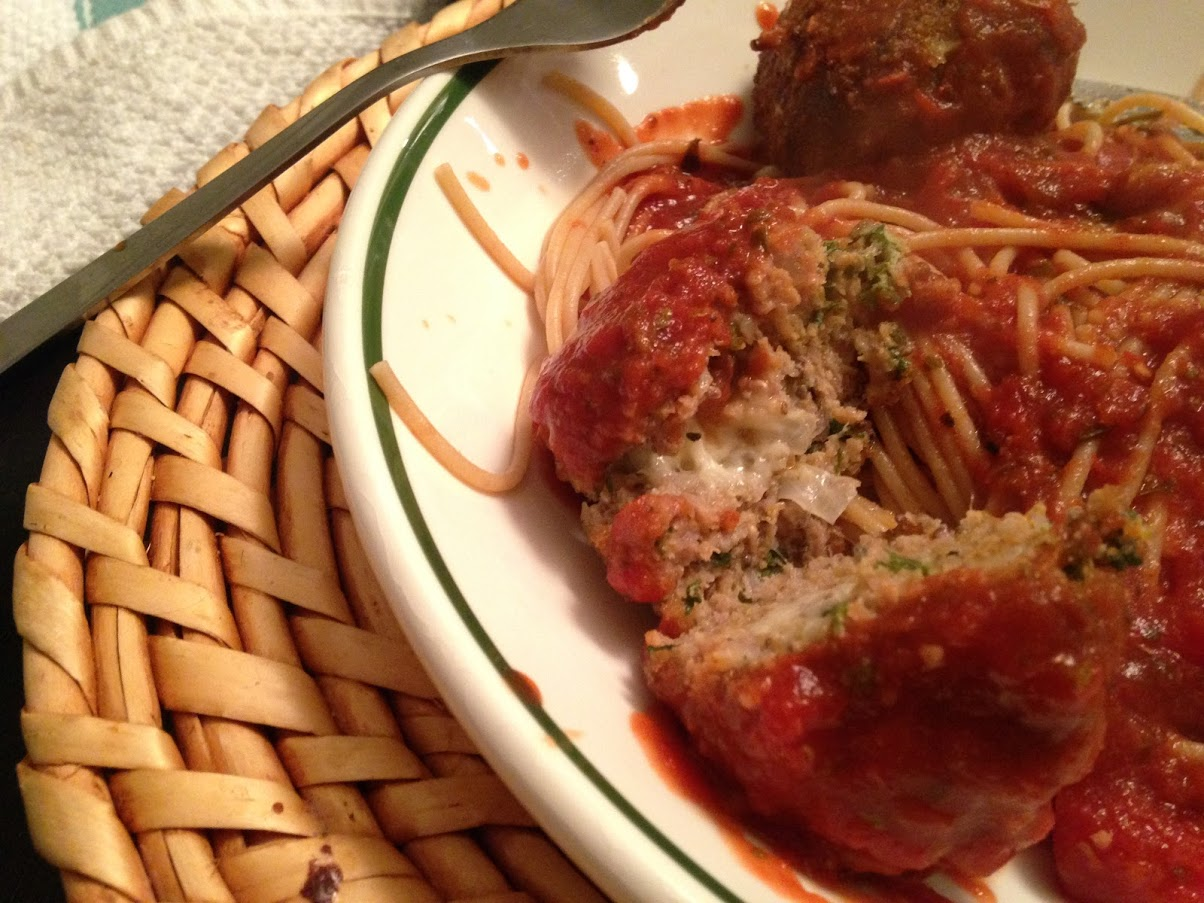
\includegraphics[width=\linewidth]{images/IMG_1095.JPG}
\end{center}
\end{figure}
\newpage
\newrecipe
\begin{recipe}
[
preparationtime = {\unit[30]{m}},
portion = {\portion{4-6}},
source = Steve
]
{Chicken Orzo}

\ingredients{
2 tablespoons butter\\ 
1 box orzo\\ 
1lb boneless skinless chicken breast\\ 
1 cup feta cheese\\ 
1 cup shredded mozzarella cheese\\ 
2-3 cups spinach\\ 
2-3 cloves minced garlic\\ 
$\frac{1}{2}$ tablespoon essence\\ 
1 teaspoon paprika\\ 
pinch of salt and pepper\\ 
}

\preparation{
\step Cook the orzo according to directions. While waiting, prepare the chicken as below. 
\step Chop the chicken into $\frac{1}{2}$ inch cubes. Heat some oil on medium-high in a pan.
\step Season the chicken with the essense, paprika, salt and pepper, then cook in pan (around 5-7 minutes).
\step Strain the orzo with a fine strainer then return it to the pot and mix in the butter and minced garlic.
\step Add the chicken, spinach, mozzarella and feta to the past mixture and mix thoroughly.
}
\end{recipe}

\newrecipe
\begin{recipe}
[
preparationtime = {\unit[45]{m}},
portion = {\portion{4-6}},
source = Steve
]
{Creamy Cajun Pasta}

\ingredients{
2 boneless skinless chicken breast\\ 
$\frac{1}{2}$ pound bacon\\ 
12-16 ounces linguine\\ 
4 teaspoons Cajun seasoning\\ 
4 tablespoons butter\\ 
1 thinly sliced green onion\\ 
1 cup heavy whipping cream\\ 
4 tablespoons chopped sun-dried tomatoes\\ 
$\frac{1}{2}$ teaspoon salt\\ 
$\frac{1}{2}$ teaspoon dried basil\\ 
$\frac{1}{4}$ teaspoon ground black pepper\\ 
1 minced garlic clove\\ 
}

\preparation{
\step Cook linguine al dente. While waiting, chop up chicken and bacon into chunks.
\step Place chicken, bacon, and Cajun seasoning in a bowl and toss to coat.
\step In a large skillet over medium heat, saut\'{e} chicken and bacon in butter or margarine until chicken is tender, about 5 to 7 minutes.
\step Reduce heat and add green onion, heavy cream, tomatoes, basil, salt, minced garlic, black pepper and heat through.
\step Pour over hot linguine and toss with Parmesan cheese.
}
\end{recipe}

\newrecipe
\begin{recipe}
[
preparationtime = {\unit[20]{m}},
portion = {\portion{4-6}},
source = Mom's
]
{Fettuccine Alfredo}

\ingredients{
6 ounces fettuccine, uncooked\\ 
$\frac{1}{4}$ cup butter\\ 
2 tablespoons flour\\ 
$\frac{1}{2}$ cup half and half\\ 
$\frac{1}{2}$ cup water\\ 
$\frac{1}{2}$ cup freshly grated Parmesan cheese\\ 
2 teaspoons parsley flakes\\ 
$\frac{1}{2}$ teaspoon coarsely ground pepper\\ 
$\frac{1}{4}$ teaspoon salt\\ 
1/8 teaspoon essence\\ 
1 glove garlic, minced\\ 
}

\preparation{
\step Cook fettuccine according to package directions, strain.
\step Melt butter in a heavy saucepan over low heat, add flour whisk for 2 minutes to make a white roux. Gradually add half and half and water, cook over medium heat, stirring constantly until mixture is thickened and bubbly. This makes the B\'echamel sauce.
\step Stir in Parmesan cheese, and remaining ingredients. Toss with fettuccine. Serve immediately.
}
\end{recipe}

\newrecipe
\begin{recipe}
[
preparationtime = {\unit[40]{m}},
bakingtime = {\unit[30]{m}},
portion = {\portion{4-6}},
source = Giada De Laurentis with changes by Mom
]
{Italian Baked Chicken and Pastina}

\ingredients{
2 cups pastina pasta (or any small pasta)\\ 
2 tablespoons olive oil\\ 
1 cup cubed chicken breast\\ 
$\frac{1}{2}$ cup diced onion\\ 
1 clove garlic, minced\\ 
2 (14.5 ounce) cans diced tomatoes\\ 
%(Delmonte diced tomatoes with garlic, basil and olive oil)
%(Mom puts them in the blender and chops them to make more of a sauce)
2 cups shredded mozzarella\\ 
$\frac{1}{4}$ cup chopped fresh flat leaf parsley\\ 
$\frac{1}{2}$ teaspoon kosher salt\\ 
$\frac{1}{2}$ teaspoon fresh ground pepper\\ 
$\frac{1}{4}$ cup bread crumbs\\ 
$\frac{1}{4}$ cup grated parmesan\\ 
1$\frac{1}{2}$ tablespoon butter\\ 
}

\hint{Mom recommends using Delmonte diced tomatoes with garlic, basil and olive oil and putting them in the blender to chop them up into more of a sauce.}

\preparation{
\step Preheat oven to 400 degrees. Use $\frac{1}{2}$ tablespoon of the butter to butter a 8x8x2 inch baking dish.
\step Bring a medium pot of salted water to a boil over high heat. Add the pasta and cook until tender, stirring occasionally about 7-8 minutes.
\step Drain pasta into a large mixing bowl.\\ 
\step Meanwhile put the olive oil in a medium saut\'{e} pan over medium heat. Add the chicken and cook for 3 minutes.
\step Add the onion and garlic, stirring to combine and cook until the onions are soft and the chicken cooked through, about 5 minutes more.
\step Put the chicken mixture into the bowl with the cooked pasta. Add the canned tomatoes, mozzarella cheese, parsley, salt and pepper.
\step Stir to combine. Then, place the mixture in the buttered baking dish.\\ 
\step Sprinkle the bread crumbs and parmesan cheese over the top of the pasta mixture. Dot the top with small bits of 1 tablespoon of the butter.
\step Bake until the top is golden brown, about 30 minutes.
}
\end{recipe}

\newrecipe
\begin{recipe}
[
preparationtime = {\unit[1]{h}},
bakingtime = {\unit[45]{m}},
portion = {\portion{4-6}},
]
{Lasagna}

\ingredients{
1 pound ground beef\\ 
1 small onion, diced\\ 
1 28 ounce can tomatoes\\ 
1 12 ounce can tomato paste\\ 
1 tablespoon sugar\\ 
1 $\frac{1}{2}$ teaspoons salt\\ 
$\frac{1}{2}$ teaspoon oregano\\ 
$\frac{1}{2}$ teaspoon thyme\\ 
$\frac{1}{2}$ teaspoon crushed red pepper\\ 
1 garlic glove\\ 
1 bay leaf\\ 
16 ounce lasagna noodles\\ 
2 eggs\\ 
15 ounce ricotta cheese\\ 
16 ounce shredded mozzarella cheese\\ 
}

\preparation{
\step In a 5 quart dutch oven over high heat, cook ground beef and onion until pan juices evaporate and beef is browned.
\step Add tomatoes, their liquid and next 8 ingredients (tomato paste, sugar, salt, oregano, thyme, red pepper, garlic, and bay leaf).
\step Heat mixture to boiling, stirring to break up tomatoes. Reduce heat to low, cover and simmer 30 minutes, stirring mixture occasionally.
\step Discard bay leaf. Tilt pan and spoon off any fat which accumulates on top of sauce.
\step Cook lasagna noodles as label directs; drain well in colander.
\step In 13x9 inch baking dish, arrange half of drained lasagna noodles overlapping to fit. 
\step Preheat oven to 375 degrees.\\ 
\step In a small bowl with spoon, combine eggs and ricotta cheese and spoon one half of this mixture over lasagna noodles in baking dish.
\step Sprinkle with one half mozzarella; top with one half sauce. Repeat layers. Bake in oven 45 minutes. 
\step Remove from oven and let stand 10 minutes before serving.
}
\end{recipe}

\begin{recipe}
[
preparationtime = {\unit[40]{m}},
bakingtime = {\unit[40]{m}},
portion = {\portion{5-7}},
source = Emeril Lagasse
]
{Macaroni and 4 Cheeses}

\ingredients{
7 tablespoons butter\\ 
4 tablespoons flour\\ 
2 cups half \& half\\ 
$\frac{3}{4}$ teaspoon salt\\ 
$\frac{1}{4}$ teaspoon pepper\\ 
$\frac{1}{4}$ teaspoon red hot sauce\\ 
8-1/2 ounces graded parmigiano-reggiano\\ 
1 pound elbow macaroni\\ 
$\frac{1}{2}$ teaspoon minced garlic\\ 
4 ounces grated cheddar cheese\\ 
4 ounces grated fontina cheese\\ 
4 ounces grated gruyere cheese\\ 
$\frac{1}{4}$ cup fresh bread crumbs\\ 
$\frac{1}{2}$ teaspoon essence\\ 
}

\hint{Make sure to use good quality cheese, especially the parmesan and cheddar, I like to use a good white cheddar. Gruyere can be substituted with other high quality swiss cheeses and fontina can be substituted as well according to taste.\\ 
For lobser mac and cheese, add 1$\frac{1}{2}$ to 2 lbs of cooked lobster meat (or any other type of meat can be added).}

\preparation{
\step Grate fontina, gruyere cheese, cheddar, and parmigiano-reggiano (keep 4 ounces of this separate.
\step  In large bowl combine remaining parmesan cheese (4.5 ounces), cheddar, fontina, and gruyere.
\step Boil pot of water, cook macaroni as directed -- drain in colander and return the macaroni to the pot.
\step Add 2 tablespoons butter and fresh chopped garlic to the macaroni and stir to combine.
\step In a separate pot, heat 4 tablespoons butter and melt then add flour and cook 3 minutes whisking until a white roux develops.
\step Stir in half \& half little by little -- 4 to 5 minutes until it begins to get thick, creating a b\'echamel sauce.
\step Season b\'echamel sauce with salt, pepper and hot sauce and add 4 ounces of grated parmesan that was set aside. Stir until cheese is melted and smooth
\step Add b\'{e}chamel sauce to the macaroni and stir until well combined.\\ 
\step Using the remaining tablespoon of butter, grease a 3 quart baking dish or casserole and preheat oven to 350 degrees.
\step Place one-third of the macaroni in the bottom of the prepared baking dish. Top with one-third of the mixed cheeses.
\step Top with another third of the macaroni and another third of the cheese mixture.\\ 
\step Repeat with the remaining macaroni and cheese mixture. Sprinkle the bread crumbs and essence over the top.
\step Bake for 30 to 45 minutes or until the macaroni and cheese is bubbly and hot and the top is golden brown. Remove from the oven and let sit 5 minutes before serving.
% (For lobser mac and cheese, add 1$\frac{1}{2}$ to 2 lbs of cooked lobster meat)
}
\end{recipe}

\newrecipe
\begin{recipe}
[
preparationtime = {\unit[1]{h}},
bakingtime = {\unit[30]{m}},
portion = {\portion{4-5}},
]
{Manicotti}

\ingredients{
Sauce\\ 
1 cup all purpose flour\\ 
4 eggs\\ 
1 tablespoon oil\\ 
1 teaspoon salt\\ 
1 cup water\\ 
2 cups ricotta cheese\\ 
2 tablespoons grated parmesan cheese\\ 
$\frac{3}{4}$ teaspoon salt\\ 
$\frac{1}{4}$ teaspoon pepper\\ 
2 eggs\\ 
8 ounces mozzarella cheese, coarsely shredded\\ 
}

\preparation{
\step Prepare marinara sauce (add meat if desired).\\ 
\step For manicotti noodles, in a small bowl with mixer at low speed, blend flour, eggs, oil, salt and water at medium speed, beat 1 minute.
\step Lighlty brush 7 inch skillet with oil. Over medium high heat, heat skillet.
\step Pour in about 2 tablespoons  batter; tip pan to coat bottom evenly with batter. Cook until the top is set and dry and underside lightly browned, about 30 seconds. Lift noodle onto waxed paper. Repeat.
\step Spoon 1/3 of hot sauce evenly into 1 15 $\frac{1}{2}$ by 10 $\frac{1}{2}$ inch roasting pan.
\step In medium bowl, mix ricotta cheese, Parmesan cheese, salt, pepper, and eggs until well blended.
\step Add mozzarella and stir. Then preheat oven to 375 degrees.\\ 
\step Spoon heaping tablespoon of cheese mixture down center of each noodle.\\ 
\step Fold noodle edges over cheese to form manicotti. Arrange filled noodle seam side down in roasting pan.
\step Spoon remaining sauce over noodles. Bake 30 minutes or until sauce is hot and bubbly.
}
\end{recipe}

\newrecipe
\begin{recipe}
[
preparationtime = {\unit[1]{h}},
bakingtime = {\unit[45]{m}},
portion = {\portion{5-7}},
source = Emeril
]
{Penne a La Vodka Casserole}

\ingredients{
4 tablespoons extra virgin olive oil\\ 
1 pound sweet Italian sausage\\ 
%, cut crosswise into 1 inch slices
1 pound hot Italian sausage\\
%, cut crosswise into 1 inch slices
4 cups thinly sliced onions\\ 
1 $\frac{3}{4}$ = teaspoons salt\\ 
$\frac{3}{4}$ teaspoon freshly ground black pepper\\ 
$\frac{1}{4}$ cup thinly sliced fresh basil leaves\\ 
1 tablespoon minced garlic\\ 
$\frac{1}{2}$ cup vodka\\ 
2 (16 ounce) cans crushed tomatoes w/ juice\\ 
1 teaspoon essence\\ 
$\frac{1}{2}$ cup heavy cream\\ 
1 tablespoon olive oil\\ 
1 pound penne pasta\\ 
15 ounces ricotta\\ 
1 cup grated parmigaino-reggiano\\ 
1 $\frac{1}{2}$ cups grated mozzarella\\ 
}

\preparation{
\step Preheat oven to 350 degrees. Then cut sausages crosswise into 1 inch slices.
\step Heat 2 tablespoons extra virgin olive oil in large skillet over high heat. Add the sausage and cook stirring until browned, 4 to 5 minutes.
\step Add the onions, $\frac{3}{4}$ teaspoon salt and the black pepper.
\step Cook, stirring occasionally until the onions are just soft about 4 minutes.
\step Add the basil and garlic and cook, stirring for 2 minutes. Then Add the vodka and tomatoes, reduce the heat to medium-low and simmer, uncovered stirring occasionally for 40 minutes.
\step Add the essence and heavy cream, stir to mix and simmer for 5 minutes. Then, remove from the heat.
\step To cook the pasta, combine 4 quarts water, the 1 tablespoon olive oil and the remaining 1 teaspoon of salt in the large pot over high heat. Bring to the boil, add the pasta and cook 14-15 minutes.
\step Remove from the heat and drain well. Combine half of the ricotta cheese and half of the Parmigiano-Reggiano with the remaining 2 tablespoons extra-virgin olive oil in a large mixing bowl.
\step Add the pasta and toss to coat evenly. Add the sausage mixture and mix well. Add the remaining Parmigiano-Reggiano and mix well.
\step Transfer the mixture to a 9 by 13 inch baking dish. Sprinkle with the mozzarella and bake until bubbly and golden about 45 minutes.
\step Remove from the oven. Serve warm.
}
\end{recipe}

\newrecipe
\begin{recipe}
[
preparationtime = {\unit[1]{h}},
bakingtime = {\unit[45]{m}},
portion = {\portion{5-7}},
source = Giada De Laurentis
]
{Penne with Shrimp and Herbed Cream Sauce}

\ingredients{
1 pound penne pasta\\ 
$\frac{1}{4}$ cup olive oil\\ 
1 pound medium shrimp, peeled/deveined\\ 
4 cloves garlic, minced\\ 
$\frac{1}{2}$ teaspoon kosher salt\\ 
$\frac{1}{2}$ teaspoon freshly ground black pepper\\ 
1 (15 ounce can) chopped tomatoes\\ 
%  (Delmonte olive oil, garlic \& basil)
$\frac{1}{2}$ cup chopped fresh basil leaves\\ 
$\frac{1}{2}$ cup chopped fresh flat leaf parsley\\ 
$\frac{1}{4}$ teaspoon crushed red pepper flakes\\ 
1 cup white wine\\ 
1/3 cup clam juice\\ 
$\frac{3}{4}$ cup whipping cream\\ 
$\frac{1}{2}$ cup grated Parmesan\\ 
}

\preparation{
\step Bring to a large pot of salted water to a boil over high heat. Add the pasta and cook until tender. Then drain the pasta and set aside.
\step In a large skillet, heat the oil over medium high heat. Add the shrimp, garlic, $\frac{1}{2}$ teaspoon of salt, and $\frac{1}{2}$ teaspoon of pepper. 
\step Cook, stirring frequently until the shrimp turn pink and are cooked through, about 3 minutes. 
\step Using a slotted spoon, remove the shrimp from the pan and set aside.
\step Add the tomatoes, $\frac{1}{4}$ cup basil, $\frac{1}{4}$ cup parsley and the red pepper flakes. Cook for 2 minutes, stirring constantly.
\step Add the wine, clam juice, and heavy cream. Bring the mixture to a boil.
\step Reduce the heat to medium-low and simmer for 7 to 8 minutes until the sauce thickens.
\step Add $\frac{1}{4}$ cup of the Parmesan, the cooked shrimp, the cooked pasta and the remaining herbs. Toss together until all ingredients are coated. 
\step Season to taste with extra salt and pepper. Then, transfer the pasta to a large serving bowl. Sprinkle with the remaining cheese and serve.
}
\end{recipe}

\newrecipe
\begin{recipe}
[
preparationtime = {\unit[40]{m}},
portion = {\portion{4-5}},
source = Steve
]
{Spaghetti and Meatballs}

\ingredients{
1 pound spaghetti\\ 
sprinkle of salt\\ 
\textbf{For the Meatballs:}\hspace*{\hfill}\\ 
1 pound ground Italian sausage\\ 
$\frac{1}{2}$ chopped white onion\\ 
2 teaspoons Worcestershire sauce\\ 
1 egg, beaten\\ 
$\frac{1}{2}$ cup Italian bread crumbs\\ 
$\frac{1}{4}$ cup grated Parmesan\\ 
%, Parmigiano-Reggiano or Romano cheese
2 cloves garlic, chopped\\ 
Salt and pepper\\ 
\textbf{For the sauce:}\hspace*{\hfill}\\ 
2 tablespoons extra-virgin olive oil\\ 
$\frac{1}{2}$ teaspoon paprika\\ 
4 cloves garlic, crushed or chopped\\ 
1 small onion, finely chopped\\ 
$\frac{1}{2}$ cup beef stock\\ 
$\frac{1}{2}$ cup red wine\\ 
1 (28-ounce) can crushed tomatoes\\ 
A handful chopped flat-leaf parsley\\ 
10 leaves fresh basil leaves\\ 
%, torn or thinly sliced
}

\hint{For a smoother sauce, you can pulse blend the sauce ingredients before cooking.}

\preparation{
\step Place a large pot of water (sprinkled with salt) to boil. When it boils, add pasta and cook to al dente.
\step In a bowl, mix sausage, Worcestershire, egg, white onion, bread crumbs, cheese, garlic, salt and pepper.
\step Hand roll meat into 1 1/2 inch medium-sized meatballs.
\step Heat a small amount of oil in a large sauce pan up to medium-high. Then add the meatballs and, turning them to brown all sides.
\step Make the sauce on the meatballs by adding oil, crushed pepper, garlic and finely chopped onion. Saute 5 to 7 minutes, until onion bits are soft.
\step Add the beef stock, wine, crushed tomatoes, and herbs. Bring to a simmer and cook on low covered for about 20 minutes.
\step Drain pasta and serve hot with a ladle of the sauce with some meatballs and grated cheese. 
}
\end{recipe}


\chapter{Pizza}
\begin{figure}[h]
\begin{center}
   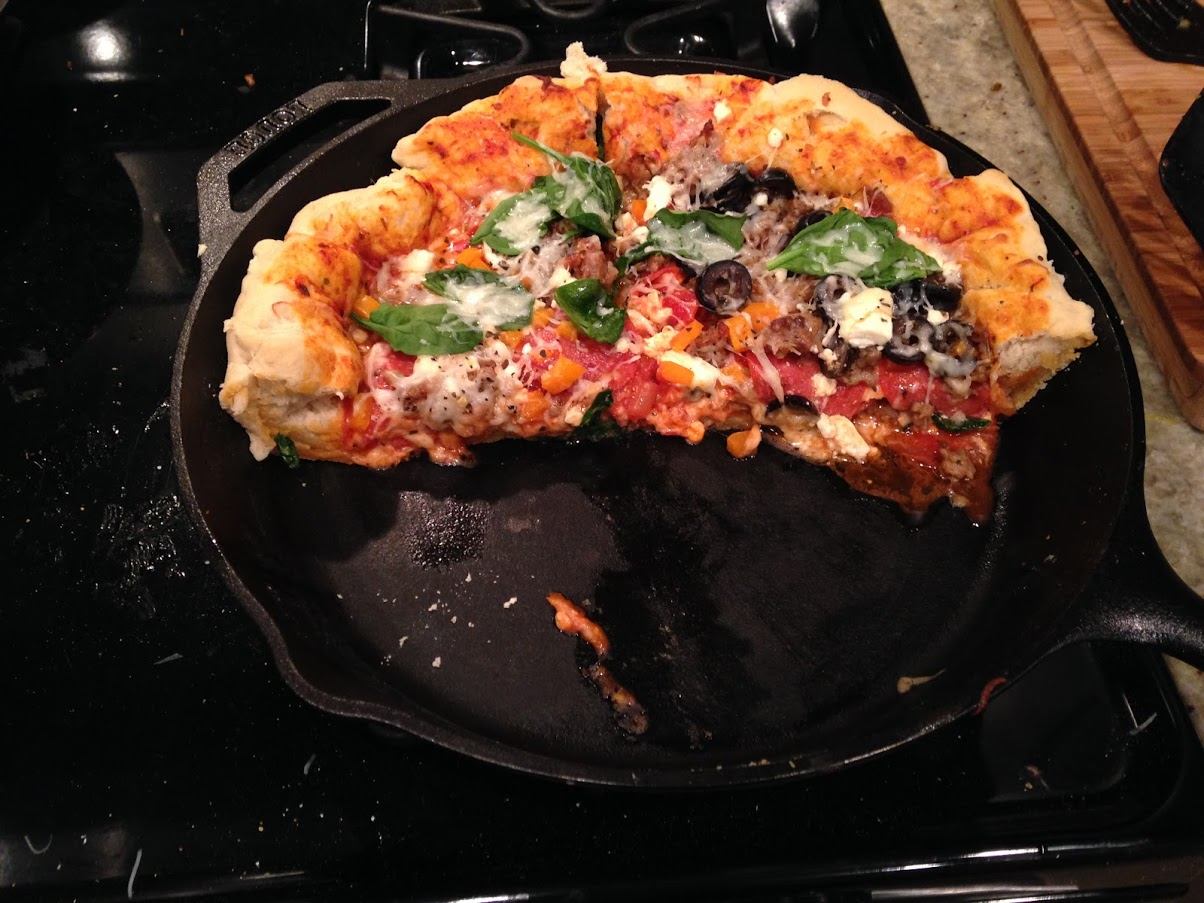
\includegraphics[width=\linewidth]{images/IMG_1083.JPG}
\end{center}
\end{figure}
\newpage
\newrecipe
\begin{recipe}
[
preparationtime = {\unit[20]{m}},
bakingtime = {\unit[10]{m}},
portion = {\portion{1}},
source = Steve
]
{Prosciutto and Arugula Pizza}

\introduction{Add one of the following cheeses to your mozzarella for an easy flavor twist:
\begin{multicols}{3}
\small \begin{itemize}
    \item Asiago
    \item Cheddar
    \item Feta
    \item Fontina
    \item Gouda
    \item Gorgonzola
    \item Parmesan
    \item Provolone
    \item Romano
\end{itemize}
\end{multicols}
}

\hint{You can use store bought dough or the Pizza dough from Page~\pageref{pg:pizza_dough}. Same with the pizza sauce in Page~\pageref{pg:pizza_sauce}}

\ingredients{
Pizza dough\\ 
$\frac{1}{2}$ cup pizza sauce\\ 
4 ounces fresh mozzarella cheese\\ 
2 ounces very thinly sliced prosciutto\\ 
$\frac{1}{2}$ tablespoon extra virgin olive oil\\ 
1$\frac{1}{3}$ cups baby arugula\\ 
}

\suggestion{You can modify this pizza recipe for any toppings you like.}

\preparation{
\step Preheat oven to 450\degree. While waiting, spread the sauce over the crust leaving a small border.
\step Thinly slice mozzarella and spread evenly over sauce.
\step Bake pizza for 10 minutes or until bottom is lightly browned and cheese is melted then pull it out to let it cool.
\step Cut the prosciutto into $\frac{1}{2}$ inch strips and place on warm pizza. 
\step Toss the arugula with the olive oil and then evenly spread over pizza.
}
\end{recipe}

%Try some of these:
%Mozzarella, Romano, Parmesan
%Fontina, Gruyère
%Mozzarella, Parmesan, Gorgonzola
%Goat cheese, Parmesan, mozzarella
%Mozzarella, Taleggio
\newrecipe
\begin{recipe}
[
preparationtime = {\unit[15]{m}},
bakingtime = {\unit[20]{m}},
portion = {\portion{2-4}},
source = Mom with changes by Steve
]
{Stromboli}

\hint{You can use store bought dough or the Pizza dough from Page~\pageref{pg:pizza_dough}. Same with the pizza sauce in Page~\pageref{pg:pizza_sauce}}

\ingredients{
Pizza dough\\ 
% (refrigerator, fresh or frozen-defrosted)
1 jar marinara or fresh sauce\\ 
Italian sausage\\ 
$\frac{1}{2}$ white onion\\
$\frac{1}{2}$ bell pepper\\
Pepperoni\\ 
Black olives\\ 
1 cup shredded Mozzarella cheese\\ 
1 cup shredded Cheddar or Asiago cheese\\ 
Handful of Feta cheese\\ 
Anything you like on pizza\\
}

\suggestion{You can modify this pizza recipe for any toppings you like.}

\preparation{
\step Brown Italian sausage. You can optionally add sliced onions and cook until soft or just add the onions in later with the rest of the ingredients.
\step Chop up the bell pepper, onion, and black olives (as well as whatever other ingredients you desire).
\step Roll dough into a rectangle. Add Italian sausage, pepperoni, onions, bell peppers, and black olives. Then sprinkle cheeses evenly over top.
\step Roll up the dough lengthwise into a jelly roll. Fold over the edges and pinch all seals.
\step Lay Stromboli on rectangle plan seal side down after lightly coating the pan with butter or oil. 
\step Cook 375 degrees for 20-25 minutes depending on dough type.
\step Heat sauce and serve with Stromboli.
}
\end{recipe}


\part{Soups, Salads, and Sauces}

\chapter{Soups}
\begin{figure}[h]
\begin{center}
   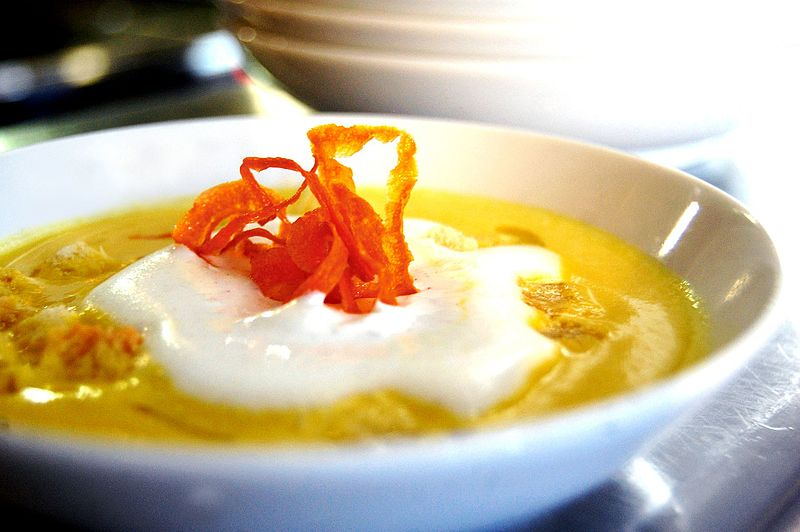
\includegraphics[width=0.9\linewidth]{images/800px-Butternut_squash_soup.jpg}
\end{center}
\end{figure}
\newpage
\newrecipe
\begin{recipe}
[
preparationtime = {\unit[35]{m}},
bakingtime = {\unit[3]{h}},
portion = {\portion{4-6}},
]
{Beef and Guinness Stew}

\ingredients{
2 pounds stewing beef\\ 
3 tablespoons oil\\ 
2 tablespoons flour\\ 
Salt and freshly ground black pepper\\ 
Pinch of cayenne\\ 
2 large onions, coarsely chopped\\ 
1 garlic clove, crushed\\ 
2 tablespoons tomato puree\\ 
%, dissolved in 4 tablespoons water
1 $\frac{1}{4}$ cups Guinness\\ 
2 cups largely diced carrots\\ 
Sprig of fresh thyme\\ 
Chopped parsley, for garnish\\ 
}

\preparation{
\step Trim the meat of any fat or gristle and cut into 2 inch cubes. Toss beef with 1 tablespoon of the oil.
\step In a small bowl, season the flour with salt, pepper and cayenne. Toss meat with seasoned flour.
\step Heat remaining 2 tablespoons oil in a large skillet over high heat. Brown the meat on all sides.
\step Dissolve the tomato puree into 4 tablespoons of water, mixing well. 
\step Reduce the heat, add the onions, crushed garlic and tomato puree to the skillet, cover and cook gently for 5 minutes.
\step Transfer the contents of the skillet to a casserole and pour half of the Guinness into the skillet. 
\step Bring Guinness to a boil and stir to dissolve the caramelized meat juices on the pan.
\step Pour over the meat, along with the remaining Guinness. Add the carrots and thyme.\\ 
\step Stir and adjust seasonings. Cover the casserole and simmer over low heat or in a 300 degree oven until the meat is tender 2 to 3 hours. 
\step Garnish the beef with parsley.
}
\end{recipe}

\newrecipe
\begin{recipe}
[
preparationtime = {\unit[40]{m}},
bakingtime = {\unit[55]{m}},
portion = {\portion{4-6}},
]
{Roasted Pear-Butternut Soup with Crumbled Stilton}

\ingredients{
2 ripe pears\\ 
%, peeled, quartered and cored\\ 
2 pounds butternut squash\\ 
%, peeled, seeded and cut into 2 inch chunks\\ 
2 medium tomatoes, cored and quartered\\ 
1 large leek\\ 
%, pale green and white parts only, halved lengthwise, sliced and washed thoroughly
2 cloves garlic crushed\\ 
2 tablespoons extra-virgin olive oil\\ 
$\frac{1}{2}$ teaspoon salt\\ 
Freshly ground pepper\\ 
4 cups vegetable broth\\ 
$\frac{2}{3}$ cup crumbled Stilton or blue cheese\\ 
1 tablespoon thinly sliced fresh chives\\ 
}

\preparation{
\step Preheat oven to 400 degrees. Then peel, core, and quarter the pears.
\step De-seed the butternut squash, peel and cut it into 2 inch chunks.
\step Take only the pale green and white parts of the leek, half lengthwise, slice and washed thoroughly.
\step Combine pears, squash, tomatoes, leek, garlic, oil, $\frac{1}{4}$ teaspoon salt and pepper in a large bowl; toss to coat.
\step Spread the mixture evenly on a large rimmed baking sheet. Roast, stirring occasionally, until the vegetables are tender, 40 to 55 minutes. Let cool slightly.
\step Place half the vegetables and 2 cups broth in a blender, puree until smooth. Transfer to a large saucepan.
\step Puree the remaining vegetables and 2 cups broth. Add to the pan and stir in the remaining $\frac{1}{4}$ teaspoon salt.
\step Cook the soup over medium low heat, stirring until hot, about 10 minutes. Divide among 6 bowls and garnish with cheese and chives.
}
\end{recipe}

\newrecipe
\begin{recipe}
[
preparationtime = {\unit[50]{m}},
portion = {\portion{4}},
]
{Lasagna Soup}

\ingredients{
Kosher salt\\ 
8 ounces lasagna noodles (about 10 noodles)\\ 
1 tablespoon extra virgin olive oil\\ 
%plus more for drizzling
1 onion, chopped\\ 
$\frac{1}{2}$ pound sweet Italian sausage, casing removed\\ 
3 cloves garlic, chopped\\ 
1 teaspoon dried oregano\\ 
2 tablespoons tomato paste\\ 
4 cups low sodium chicken broth\\ 
1 15 ounce can crushed tomatoes\\ 
$\frac{1}{2}$ cup chopped fresh basil\\ 
Extra basil leaves for topping\\ 
$\frac{1}{3}$ cup grated parmesan cheese\\ 
$\frac{1}{4}$ cup heavy cream or half and half\\ 
Ricotta cheese for topping\\ 
}

\preparation{
\step Bring a large pot of salted water to a boil. While waiting, break lasagna noodles into pieces.
\step Add the noodles and cook as the label directs. Drain, drizzle with the olive oil and toss.
\step Heat 1 tablespoon olive oil in a large dutch oven or heavy bottomed pot over medium high heat.
\step Add the onion and cook stirring until softened about 4 minutes.
\step Add the sausage, garlic and oregano and cook, stirring and breaking up the sausage with a wooden spoon until the sausage is browned, about 3 minutes.
\step Add the tomato paste and cook stirring until darkened about 2 minutes.
\step Add the chicken broth, tomatoes, and 1 cup water, cover and bring to a simmer.
\step Uncover and cook until slightly reduced about 10 minutes.
\step Stir in the noodles, basil, parmesan and heavy cream, simmer 2 more minutes.\\ 
\step Divide the soup among bowls. Top with ricotta and sliced basil.
}
\end{recipe}

\chapter{Sauces}
\begin{figure}[h]
\begin{center}
   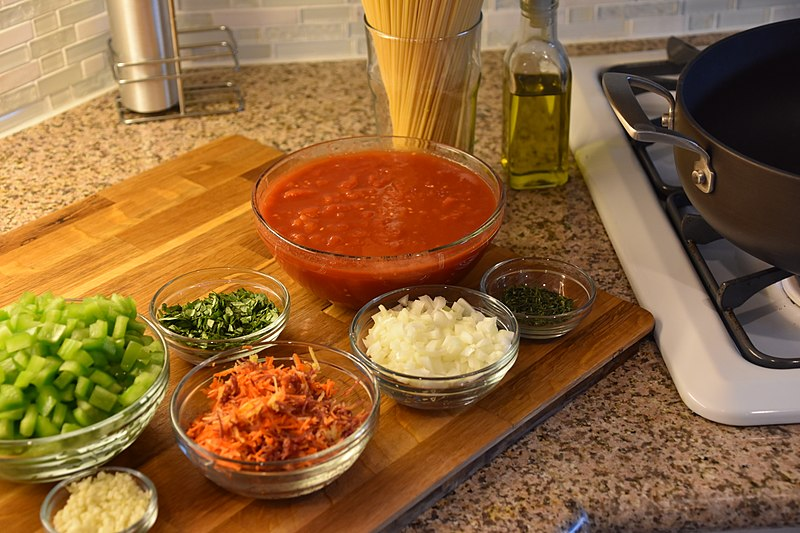
\includegraphics[width=\linewidth]{images/800px-Making_Spaghetti_Sauce.jpg}
\end{center}
\end{figure}
\newpage
\newrecipe
\begin{recipe}
[
preparationtime = {\unit[40]{m}},
portion = {\portion{2}},
source = Steve
]
{Pizza Sauce}\label{pg:pizza_sauce}

\ingredients{
2 tablespoons olive oil\\ 
1 clove garlic, minced\\ 
28 oz. can crushed tomatoes\\ 
6 oz. can tomato paste\\ 
$\frac{1}{2}$ tablespoon sugar\\ 
$\frac{3}{4}$ teaspoon salt\\ 
1 teaspoon basil\\ 
$\frac{1}{2}$ teaspoon dried oregano\\ 
Freshly cracked pepper\\ 
Pinch crushed red pepper\\ 
}

\preparation{
\step Lightly pulse blend the crushed tomatoes, tomato paste, sugar, salt, basil, oregano, some freshly cracked pepper (10-15 cranks of a pepper mill), and a pinch of red pepper flakes to combine.
\step Add the olive oil and garlic to a sauce pot and cook over medium heat for 1-2 minutes, or just until the garlic is soft and fragrant.
\step Add the blended mixture to the oil in the sauce pot and mix together.
\step Cover the pot, allow to come to a simmer, then reduce the heat to low and let simmer for 15 to 30 minutes.
}
\end{recipe}

\newrecipe
\begin{recipe}
[
preparationtime = {\unit[20]{m}},
portion = {\portion{2-3}},
]
{Bearnaise Sauce}

\ingredients{
3 tablespoons white wine vinegar\\ 
3 tablespoons dry white wine\\ 
10 peppercorns, crushed\\ 
3 shallots, finely chopped\\ 
1 tablespoon chopped fresh tarragon\\ 
1 tablespoon water\\ 
3 egg yolks\\ 
$\frac{1}{4}$ teaspoon salt\\ 
Pinch of ground red pepper\\ 
$\frac{3}{4}$ cup unsalted butter, melted and cooled\\ 
1 tablespoon chopped fresh parsley\\
% chervil or parsley
}

\preparation{
\step Bring the first 5 ingredients to a boil over medium high heat (white wine vinegar, white wine, peppercorns, shallots, and tarragon), and cook whisking constantly until mixture is reduced to 1 tablespoon.
\step Remove from heat and whisk in water and next 3 ingredients (egg yolks, salt, and red pepper).
\step Cook over low heat, whisking constantly, about 4 minutes or until pale yellow. Remove from heat.
\step Add butter in slow, steady stream, whisking constantly until thickened.
\step Pour sauce through a wire mesh strainer into a bowl, discarding shallot.
\step Stir in parsley and serve warm with steak.
}
\end{recipe}

\newrecipe
\begin{recipe}
[
preparationtime = {\unit[55]{m}},
portion = {\portion{2-3}},
source = Grandma
]
{French Dressing}

\ingredients{
$\frac{1}{4}$ cup vinegar\\ 
$\frac{1}{2}$ cup sugar\\ 
1 teaspoon dry mustard\\ 
1 teaspoon salt\\ 
1 teaspoon paprika\\ 
1 cup olive oil\\ 
}

\preparation{
\step Beat all ingredients except oil for 3 minutes, then slowly add oil while beating. Beat 3 more minutes.
}
\end{recipe}

\newrecipe
\begin{recipe}
[
preparationtime = {\unit[15]{m}},
portion = {\portion{4-5}},
]
{Sweet and Sour Sauce}

\ingredients{
1 tablespoon vegetable oil\\ 
$\frac{1}{2}$ medium onion, chopped\\ 
$\frac{1}{2}$ teaspoon grated ginger\\ 
$\frac{1}{4}$ cup finely diced pineapple\\ 
1/3 cup rice vinegar\\ 
$\frac{1}{4}$ cup ketchup\\ 
2 tablespoons chili garlic sauce\\ 
$\frac{1}{4}$ cup sugar\\ 
$\frac{1}{4}$ cup chicken broth\\ 
2 teaspoons cornstarch\\ 
}

\preparation{
\step Heat the oil in a small saucepan over medium high heat. When hot, add the onions and cook, stirring until softened about 2 minutes.
\step Add the ginger and cook, stirring constantly for 30 seconds.
\step Stir in the pineapple, vinegar, ketchup, chili garlic sauce and the sugar.
\step Bring the sauce to a simmer and cook stirring for 3 minutes. 
\step In a small bowl, whisk together the chicken broth and cornstarch until smooth. Add to the sauce mixture and bring to a boil.
\step Cook for 1 minute, remove from the heat and cool slightly.
}
\end{recipe}


\end{document}